% LaTeX source for the spanish traslation of the textbook ``How to think like a computer scientist''
% Copyright (c)  2001,2002  Allen B. Downey.
% Traslation to spanish completed by
% Andrés Becerra Sandoval
% abecerra@cic.javerianacali.edu.co


% Permission is granted to copy, distribute and/or modify this
% document under the terms of the GNU Free Documentation License,
% Version 1.1  or any later version published by the Free Software
% Foundation; with the Invariant Sections being "Contributor List",
% with no Front-Cover Texts, and with no Back-Cover Texts. A copy of
% the license is included in the section entitled "GNU Free
% Documentation License".

% This distribution includes a file named fdl.tex that contains the text
% of the GNU Free Documentation License.  If it is missing, you can obtain
% it from www.gnu.org or by writing to the Free Software Foundation,
% Inc., 59 Temple Place - Suite 330, Boston, MA 02111-1307, USA.
%

\documentclass[letterpaper,twoside,10pt]{book}
\usepackage[spanish]{babel}
\usepackage{fancyhdr}
\usepackage{graphicx}
\usepackage{makeidx}
\usepackage{ucs}
\usepackage[utf8x]{inputenc}
\usepackage{palatino}
\usepackage{url}

\newcommand{\introprog}{Introducción a la programación con Python}
\addto\captionsspanish{\renewcommand{\indexname}{Índice analítico}}

\usepackage[text={5in,7in},centering,twoside]{geometry}
\setlength{\marginparsep}{0in}
\setlength{\marginparwidth}{0in}
\setlength{\marginparpush}{0in}
\setlength{\hoffset}{-5pt}

\newcommand{\beforefig}{\vspace{1.3\parskip}}
\newcommand{\afterfig}{\vspace{-0.2\parskip}}

\newcommand{\beforeverb}{\vspace{0.6\parskip}}
\newcommand{\afterverb}{\vspace{0.6\parskip}}

\newcommand{\adjustpage}[1]{\enlargethispage{#1\baselineskip}}
\newcommand{\clearemptydoublepage}{\newpage{\pagestyle{empty}\cleardoublepage}}
\newcommand{\blankpage}{\pagestyle{empty}\vspace*{1in}\newpage}

\pagestyle{fancyplain}

\renewcommand{\chaptermark}[1]{\markboth{#1}{}}
\renewcommand{\sectionmark}[1]{\markright{\thesection\ #1}{}}

\lhead[\fancyplain{}{\bfseries\thepage}]%
      {\fancyplain{}{\bfseries\rightmark}}
\rhead[\fancyplain{}{\bfseries\leftmark}]%
      {\fancyplain{}{\bfseries\thepage}}
\cfoot{}

% turn off the rule under the header
%\setlength{\headrulewidth}{0pt}

% the following is a brute-force way to prevent the headers
% from getting transformed into all-caps
\renewcommand\MakeUppercase{}

% The following lines add a little extra space to the column
% in which the Section numbers appear in the table of contents
\makeatletter
\renewcommand{\l@section}{\@dottedtocline{1}{1.5em}{3.0em}}
\makeatother
\setcounter{tocdepth}{1}

\makeindex

%%%%%%%%%%%%% INCLUDE ONLY  %%%%%%%%%%
%\includeonly{foreword,preface,contrib,traduccion}
%\includeonly{chap00}	     % solucion de problemas
%\includeonly{chap01}        % el camino del programa
%\includeonly{chap02}        % variables, expresiones, sentencias
%\includeonly{chap03}	     % funciones
%\includeonly{chap04}	     % condicionales y recursion 
%\includeonly{chap05}	     % funciones fructíferas
%\includeonly{chap06}	     % iteracion
%\includeonly{chap07}	     % cadenas
%\includeonly{chap08}	     % listas
%\includeonly{chap09}	     % tuplas
%\includeonly{chap10}	     % diccionarios 
%\includeonly{chap11}	     % archivos y excepciones
%\includeonly{chap12}	     % clases y objetos
%\includeonly{chap13}	     % clases y funciones
%\includeonly{chap14}	     % clases y metodos
%\includeonly{chap15}	     % conjuntos de objetos
%\includeonly{chap16}	     % herencia
%\includeonly{chap17}	     % listas enlazadas
%\includeonly{chap18}        % pilas
%\includeonly{chap19}        % colas (normales y de prioridad)
%\includeonly{chap20}        % arboles
%\includeonly{app01,app02,app03,app04,fdl,gfdles}
%%%%%%%%%%%%%%%%%%%%%%%%%%%%%%%%%%%%%%


\begin{document}

%\layout
\frontmatter

%----------- portada --------------------------------------------------
\newpage
\thispagestyle{empty}
{\pagestyle{empty}\linespread{1}\parindent0pt
\vspace*{0.5cm}

\vfill 

\begin{center}
{\huge \textbf{\introprog}
\par	\vspace{5cm}{\Large \textbf{Andrés Becerra Sandoval}} 
     }

\end{center}

\vfill
\begin{flushright}
{\small
Traducción y Adaptación del libro \\
`'How to think like a computer scientist, learning with Python", \\
escrito por: \\
Allen Downey\\
Jeffrey Elkner\\
Chris Meyers\\
}
\end{flushright}

\vfill



\begin{center}

\includegraphics[scale=0.2]{illustrations/logo/LogoVerticalNegro.eps} 
\end{center}
\begin{center} {\Large Facultad de Ingeniería} \end{center}
\vfill

}

%----------------------------------------- creditos javeriana--------------------------
\pagebreak

\thispagestyle{empty}
\vfill  

\includegraphics[scale=0.2,angle=270]{illustrations/logo/LogoHorizontalNegro.eps} \\
 
\parindent0pt
{\tiny \ }

{\scriptsize 
Rector: Jorge Humberto Peláez, S.J.\\
Vicerrector Académico: Antonio de Roux\\
Vicerrector del Medio Universitario: Gabriel Jaime Pérez, S.J.\\

Facultad de Ingeniería\\
Decano Académico: Jorge Francisco Estela \\
Decana del Medio Universitario: Claudia Lucía Mora \\


Titulo:  \introprog \\
Titulo original: How to think like a computer scientist, learning with Python
Autores: Allen Downey, Jeffrey Elkner, Chris Meyers \\
Traducción y adaptación: Andrés Becerra Sandoval \\
Colección: Libro\\

ISBN: 978-958-8347-22-6 \\

Coordinador Editorial: Ignacio Murgueitio\\
Email: mignacio@javerianacali.edu.co

© Derechos Reservados\\
© Sello Editorial Javeriano\\

Correspondencia, suscripciones y solicitudes de canje:\\
Calle 18 \# 118-250\\
Santiago de Cali, Valle del Cauca\\
Pontificia Universidad Javeriana\\
Facultad de Ingeniería\\
Teléfonos: (57-2) 3218200 Exts. 233 - 518 Fax 555 2823\\
Email: abecerra@javerianacali.edu.co \\

Formato 17  x  25 cms\\
Diseño e Impresión: Multimedios PUJ Cali\\

Diseño de Carátula: 
Patricia Mejía, basada en una imagen de Ken Manheimer \\
http://myriadicity.net

Impresión: 2009
}
%-------------------copyright--------------------------------------------------
\newpage
\thispagestyle{empty}
\vspace{0.25in}

Se concede permiso para copiar, distribuir, y/o modificar este documento bajo
los terminos de la GNU Free Documentation License, Versión 1.1 o cualquier
versión posterior publicada por la Free Software Foundation; manteniendo 
sin variaciones las secciones ``Prólogo,'' ``Prefacio,'' y ``Lista de contribuidores,''
sin texto de cubierta, y sin texto de contracubierta. Una copia de la licencia
está incluida en el apéndice titulado ``GNU Free Documentation License'' y una 
traducción de ésta al español en el apéndice titulado ``Licencia de Documentación Libre de GNU''.

La GNU Free Documentation License también está disponible a través de \url{www.gnu.org}
o escribiendo a la Free Software Foundation, Inc., 59 Temple Place,
Suite 330, Boston, MA 02111-1307, USA.

La forma original de este libro es código fuente \LaTeX\  y compilarlo
tiene el efecto de generar un libro de texto en una 
repesentacion independiente del dispositivo que puede ser convertida a otros 
formatos e imprimirse.

El código  fuente \LaTeX\  para este libro y mas información sobre este proyecto
se encuentra en los sitios web:

\begin{verbatim}
      http://cic.puj.edu.co/~abecerra
      http://www.thinkpython.com
\end{verbatim}

Este libro ha sido preparado utilizando \LaTeX\ y las figuras
se han realizado con xfig.  Todos estos son programas de código
abierto, gratuito.

\vspace{0.25in}
%------informacion bibliografica -----------------------------------------------------------
\newpage
\thispagestyle{empty}

\begin{center}
\framebox{
  \begin{minipage}{11cm}
   \footnotesize 
    Downey, Allen \\
    Introducción a la programación con Python / Allen Downey, Jeffrey Elkner, Chris Meyers; 
    traducido y adaptado por Andrés Becerra Sandoval. – Santiago de Cali: Pontificia Universidad Javeriana, 
    Sello Editorial Javeriano, 2009. \\
    305 p. ; 26 cm.  \\ \\
      
    Incluye referencias bibliográficas e índice. \\ \\
       
    ISBN  978-958-8347-22-6\\ \\
     
    1. Programación (computadores electrónicos) -- Metodología 2. Python (lenguaje de programación 
    para computadores) I. Meyer, Chris II. Pontificia Universidad Javeriana (Cali) III. How to think 
    like a computer scientist: learning with python IV. Tít. \\ \\

    SCDD 005.1	\hfill						   BPUJC

   \end{minipage}
   }
\end{center}
%-------------inclusión de capítulos ----------------------------------------------------

%\newpage
\normalsize
\title{\introprog}
\author{Andrés Becerra Sandoval}
\date{Junio 2009}
%\maketitle

\chapter{Prólogo}

Por David Beazley

Como educador, investigador y autor de libros, estoy encantado de
ver la terminación de este texto. Python es un lenguaje de programación
divertido y extremadamente fácil de usar que ha ganado renombre constantemente
en los años recientes. Desarrollado hace diez años por Guido van Rossum,
la sintaxis simple de Python y su ``sabor'' se derivan, en gran
parte del ABC, un lenguaje de programación para enseñanza que se desarrolló
en los 1980s. Sin embargo, Python también fue creado para resolver
problemas reales y tiene una amplia gama de características que se
encuentran en lenguajes de programación como C++, Java, Modula-3,
y Scheme. Debido a esto, uno de las características notables de Python
es la atracción que ejerce sobre programadores profesionales, científicos,
investigadores, artistas y educadores.

A pesar de ésta atracción que ejerce en muchas comunidades diversas,
usted puede todavía preguntarse ``¿porque Python?'' o ``¿porque
enseñar programación con Python?'' Responder éstas preguntas no es
una tarea fácil— especialmente cuando la opinión popular está del
lado masoquista de usar alternativas como C++ y Java. Sin embargo,
pienso que la respuesta más directa es que la programación en Python
es simplemente más divertida y más productiva.

Cuando enseño cursos de informática, yo quiero cubrir conceptos importantes,
hacer el material interesante y enganchar a los estudiantes. Desafortunadamente,
hay una tendencia en la que los cursos de programación introductorios
dedican demasiada atención hacia la abstracción matemática y a hacer
que los estudiantes se frustren con problemas molestos relacionados
con la sintaxis, la compilación y la presencia de reglas arcanas en
los lenguajes. Aunque la abstracción y el formalismo son importantes
para los ingenieros de software y para los estudiantes de ciencias
de la computación, usar este enfoque hace la informática muy aburrida.
Cuando enseño un curso no quiero tener un grupo de estudiantes sin
inspiración. Quisiera verlos intentando resolver problemas interesantes,
explorando ideas diferentes, intentando enfoques no convencionales,
rompiendo reglas y aprendiendo de sus errores. En el proceso no quiero
perder la mitad del semestre tratando de resolver problemas sintácticos
oscuros, interpretando mensajes de error del compilador incomprensibles,
o descifrando cuál de las muchas maneras en que un programa puede
generar un error grave de memoria se está presentando.

Una de las razones del por qué me gusta Python es que proporciona
un equilibrio muy bueno entre lo práctico y lo conceptual. Puesto
que se interpreta Python, los principiantes pueden empezar a hacer
cosas interesantes casi de inmediato sin perderse en problemas de
compilación y enlace. Además, Python viene con una biblioteca grande
de módulos, que pueden ser usados en dominios que van desde programación
en la web hasta aplicaciones gráficas. Tener un foco práctico es una
gran manera de enganchar a los estudiantes y permite que emprendan
proyectos significativos. Sin embargo, Python también puede servir
como una excelente base para introducir conceptos importantes de la
informática. Puesto que Python soporta completamente procedimientos
y clases, los estudiantes pueden ser introducidos gradualmente a temas
como la abstracción procedimental, las estructuras de datos y la programación
orientada a objetos—lo que se puede aplicar después a cursos posteriores
en Java o C++. Python proporciona, incluso, varias características
de los lenguajes de programación funcionales y puede usarse para introducir
conceptos que se pueden explorar con más detalle en cursos con Scheme
y Lisp.

Leyendo, el prefacio de Jeffrey, estoy sorprendido por sus comentarios
de que Python le permita ver un ``más alto nivel de éxito y un nivel
bajo de frustración'' y que puede ``avanzar mas rápido con mejores
resultados.'' Aunque estos comentarios se refieren a sus cursos introductorios,
a veces uso Python por estas mismas razones en los cursos de informática
avanzada en la Universidad de Chicago. En estos cursos enfrento constantemente
la tarea desalentadora de cubrir un montón de material difícil durante
nueve semanas. Aunque es totalmente posible para mi infligir mucho
dolor y sufrimiento usando un lenguaje como C++, he encontrado a menudo
que este enfoque es improductivo—especialmente cuando el curso se
trata de un asunto sin relación directa con la ``programación.''
He encontrado que usar Python me permite enfocar el tema del curso
y dejar a los estudiantes desarrollar proyectos substanciales.

Aunque Python siga siendo un lenguaje joven y en desarrollo, creo
que tiene un futuro brillante en la educación. Este libro es un paso
importante en esa dirección.

\vspace{0.25in}
 
\begin{flushleft}
David Beazley \\
Universidad de Chicago, Autor de {\em Python Essential Reference} 
\par
\end{flushleft}
 	\clearemptydoublepage     % prólogo
\chapter{Prefacio}

Por Jeff Elkner

Este libro debe su existencia a la colaboración hecha posible por
Internet y el movimiento de software libre. Sus tres autores—un profesor
de colegio, un profesor de secundaria y un programador profesional—tienen
todavía que verse cara a cara, pero han podido trabajar juntos y han
sido ayudados por maravillosas personas, quienes han donado su tiempo
y energía para ayudar a hacer ver mejor este libro.

Nosotros pensamos que este libro es un testamento a los beneficios
y futuras posibilidades de esta clase de colaboración, el marco que
se ha puesto en marcha por Richard Stallman y el movimiento de software
libre.

\section*{Cómo y porqué vine a utilizar Python}

En 1999, el examen del College Board's Advanced Placement (AP) de
Informática se hizo en C++ por primera vez. Como en muchas escuelas
de Estados Unidos, la decisión para cambiar el lenguaje tenía un impacto
directo en el plan de estudios de informática en la escuela secundaria
de Yorktown en Arlington, Virginia, donde yo enseño. Hasta este punto,
Pascal era el lenguaje de instrucción en nuestros cursos del primer
año y del AP. Conservando la práctica usual de dar a los estudiantes
dos años de exposición al mismo lenguaje, tomamos la decisión de cambiar
a C++ en el curso del primer año durante el periodo escolar 1997-98
de modo que siguiéramos el cambio del College Board's para el curso
del AP el año siguiente.

Dos años después, estoy convencido de que C++ no era una buena opción
para introducir la informática a los estudiantes. Aunque es un lenguaje
de programación de gran alcance, también es extremadamente difícil
de aprender y de enseñar. Me encontré constantemente peleando con
la sintaxis difícil de C++ y sus múltiples maneras de hacer las cosas,
y estaba perdiendo muchos estudiantes, innecesariamente, como resultado.
Convencido de que tenía que haber una mejor opción para nuestras clases
de primer año, fui en busca de una alternativa a C++.

Necesitaba un lenguaje que pudiera correr en las máquinas en nuestro
laboratorio Linux, también en las plataformas de Windows y Macintosh,
que muchos de los estudiantes tienen en casa. Quería que fuese un
lenguaje de código abierto, para que los estudiantes lo pudieran usar
en casa sin pagar por una licencia. Quería un lenguaje usado por programadores
profesionales, y que tuviera una comunidad activa alrededor de él.
Tenía que soportar la programación procedimental y orientada a objetos.
Y más importante, tenía que ser fácil de aprender y de enseñar. Cuando
investigué las opciones con estas metas en mente, Python saltó como
el mejor candidato para la tarea.

Pedí a uno de los estudiantes más talentosos de Yorktown, Matt Ahrens,
que le diera a Python una oportunidad. En dos meses él no sólo aprendió
el lenguaje, sino que escribió una aplicación llamada pyTicket que
permitió a nuestro personal atender peticiones de soporte tecnológico
vía web. Sabia que Matt no podría terminar una aplicación de esa escala
en tan poco tiempo con C++, y esta observación, combinada con el gravamen
positivo de Matt sobre Python, sugirió que este lenguaje era la solución
que buscaba.

\section*{Encontrando un libro de texto}

Al decidir utilizar Python en mis dos clases de informática introductoria
para el año siguiente, el problema más acuciante era la carencia de
un libro.

El contenido libre vino al rescate. A principios del año, Richard
Stallman me presentó a Allen Downey. Los dos habíamos escrito a Richard
expresando interés en desarrollar un contenido gratis y educativo.
Allen ya había escrito un libro de texto para el primer año de informática,
{\em Como pensar como un científico de la computación}. Cuando
leí este libro, inmediatamente quise usarlo en mi clase. Era el texto
más claro y mas provechoso de introducción a la informática que había
visto. Acentúa los procesos del pensamiento implicados en la programación
más bien que las características de un lenguaje particular. Leerlo
me hizo sentir un mejor profesor inmediatamente. {\em Como pensar
como un científico de la computación con Java} no solo es un libro
excelente, sino que también había sido publicado bajo la licencia
publica GNU, lo que significa que podría ser utilizado libremente
y ser modificado para resolver otras necesidades. Una vez que decidí
utilizar Python, se me ocurrió que podía traducir la versión original
del libro de Allen (en Java) al nuevo lenguaje (Python). Aunque no
podía escribir un libro de texto solo, tener el libro de Allen me
facilitó la tarea, y al mismo tiempo demostró que el modelo cooperativo
usado en el desarrollo de software también podía funcionar para el
contenido educativo.

Trabajar en este libro, por los dos últimos años, ha sido una recompensa
para mis estudiantes y para mí; y mis estudiantes tuvieron una gran
participación en el proceso. Puesto que podía realizar cambios inmediatos,
siempre que alguien encontrara un error de deletreo o un paso difícil,
yo les animaba a que buscaran errores en el libro, dándoles un punto
cada vez que hicieran una sugerencia que resultara en un cambio en
el texto. Eso tenía la ventaja doble de animarles a que leyeran el
texto más cuidadosamente y de conseguir la corrección del texto por
sus lectores críticos más importantes, los estudiantes usándolo para
aprender informática.

Para la segunda parte del libro, enfocada en la programación orientada
a objetos, sabía que alguien con más experiencia en programación que
yo era necesario para hacer el trabajo correctamente. El libro estuvo
incompleto la mayoría del año hasta que la comunidad de software abierto
me proporcionó de nuevo los medios necesarios para su terminación.

Recibí un correo electrónico de Chris Meyers, expresando su interés
en el libro. Chris es un programador profesional que empezó enseñando
un curso de programación el año anterior, usando Python en el Lane
Community College en Eugene, Oregon. La perspectiva de enseñar el
curso llevó a Chris al libro, y él comenzó a ayudarme inmediatamente.
Antes del fin de año escolar él había creado un proyecto complementario
en nuestro Sitio Web \url{http://www.ibiblio.org/obp}, titulado {\em
Python for Fun} y estaba trabajando con algunos de mis estudiantes
más avanzados como profesor principal, guiándolos mas allá de donde
yo podía llevarlos.

\section*{Introduciendo la programación con Python}

El proceso de uso y traducción de {\em Como pensar como un científico
de la computación}, por los últimos dos años, ha confirmado la conveniencia
de Python para enseñar a estudiantes principiantes. Python simplifica
bastante los ejemplos de programación y hace que las ideas importantes
sean más fáciles de enseñar.

El primer ejemplo del texto ilustra este punto. Es el tradicional
``hola, mundo'', programa que en la versión C++ del libro se ve
así:

\begin{ccode}
   #include <iostream.h>

   void main()
   {
     cout << "Hola, mundo." << endl;
   }
\end{ccode}

en la versión Python es:

\begin{pythoncode}
    print("Hola, Mundo!")
\end{pythoncode}

Aunque este es un ejemplo trivial, las ventajas de Python salen a
la luz. El curso de Informática I, en Yorktown, no tiene prerrequisitos,
es por eso que muchos de los estudiantes, que ven este ejemplo, están
mirando a su primer programa. Algunos de ellos están un poco nerviosos,
porque han oído que la programación de computadores es difícil de
aprender. La versión C++ siempre me ha forzado a escoger entre dos
opciones que no me satisfacen: explicar el \texttt{\#include}, \texttt{void
main()}, y las sentencias \{, y \} y arriesgar a confundir o intimidar
a algunos de los estudiantes al principio, o decirles, ``No te preocupes
por todo eso ahora; lo retomaré más tarde,'' y tomar el mismo riesgo.
Los objetivos educativos en este momento del curso son introducir
a los estudiantes la idea de sentencia y permitirles escribir su primer
programa. Python tiene exactamente lo que necesito para lograr esto,
y nada más.

Comparar el texto explicativo de este programa en cada versión del
libro ilustra más de lo que esto significa para los estudiantes principiantes.
Hay trece párrafos de explicación de ``Hola, mundo!'' en la versión
C++; en la versión Python, solo hay dos. Aún mas importante, los 11
párrafos que faltan no hablan de ``grandes ideas'' en la programación
de computadores, sino de minucias de la sintaxis de C++. Encontré
la misma situación al repasar todo el libro. Párrafos enteros desaparecían
en la versión Python del texto, porque su sencilla sintaxis los hacía
innecesarios.

Usar un lenguaje de muy alto nivel, como Python, le permite a un profesor
posponer los detalles de bajo nivel de la máquina hasta que los estudiantes
tengan el bagaje que necesitan para entenderlos. Permite ``poner
cosas primero'' pedagógicamente. Unos de los mejores ejemplos de
esto es la manera en la que Python maneja las variables. En C++ una
variable es un nombre para un lugar que almacena una cosa. Las variables
tienen que ser declaradas con tipos, al menos parcialmente, porque
el tamaño del lugar al cual se refieren tiene que ser predeterminado.
Así, la idea de una variable se liga con el hardware de la máquina.
El concepto poderoso y fundamental de variable ya es difícil para
los estudiantes principiantes (de informática y álgebra). Bytes y
direcciones de memoria no ayudan para nada. En Python una variable
es un nombre que se refiere a una cosa. Este es un concepto más intuitivo
para los estudiantes principiantes y está más cerca del significado
de ``variable'' que aprendieron en los cursos de matemática del
colegio. Yo me demoré menos tiempo ayudándolos con el concepto de
variable y en su uso este año, que en el pasado.

Otro ejemplo de cómo Python ayuda en la enseñanza y aprendizaje de
la programación es su sintaxis para las funciones. Mis estudiantes
siempre han tenido una gran dificultad comprendiendo las funciones.
El problema principal se centra alrededor de la diferencia entre una
definición de función y un llamado de función, y la distinción relacionada
entre un parámetro y un argumento. Python viene al rescate con una
bella sintaxis. Una definición de función empieza con la palabra clave
\texttt{def}, y simplemente digo a mis estudiantes: ``cuando definas
una función, empieza con \texttt{def}, seguido del nombre de la función
que estás definiendo, cuando llames una función, simplemente llama
(digita) su nombre.'' Los parámetros van con las definiciones y los
argumentos van con los llamados. No hay tipos de retorno, tipos para
los parámetros, o pasos de parámetro por referencia y valor, y ahora
yo puedo enseñar funciones en la mitad de tiempo que antes, con una
mejor comprensión.

Usar Python ha mejorado la eficacia de nuestro programa de informática
para todos los estudiantes. Veo un nivel general de éxito más alto
y un nivel más bajo de frustración, de lo que ya había experimentado
durante los dos años que enseñé C++. Avanzo más rápido y con mejores
resultados. Más estudiantes terminan el curso con la habilidad de
crear programas significativos; esto genera una actitud positiva hacia
la experiencia de la programación.

\section*{Construyendo una comunidad}

He recibido correos electrónicos de todas partes del mundo, de personas
que están usando este libro para aprender o enseñar programación.
Una comunidad de usuarios ha comenzado a emerger, y muchas personas
han contribuido al proyecto mandando materiales a través del sitio
Web complementario:

\begin{center}
	\url{http://www.thinkpython.com}
\end{center}

Con la publicación del libro, en forma impresa, espero que continúe
y se acelere el crecimiento de esta comunidad de usuarios.

La emergencia de esta comunidad y la posibilidad que sugiere para
otras experiencias de colaboración similar entre educadores han sido
las partes más excitantes de trabajar en este proyecto, para mí. Trabajando
juntos, nosotros podemos aumentar la calidad del material disponible
para nuestro uso y ahorrar tiempo valioso.

Yo les invito a formar parte de nuestra comunidad y espero escuchar
de ustedes. Por favor escriba a los autores a \texttt{\url{feedback@thinkpython.com}}.

\vspace{0.25in}
 
\begin{flushleft}
Jeffrey Elkner\\
Escuela Secundaria Yortown\\
Arlington, Virginia.\\
\par
\end{flushleft}  	\clearemptydoublepage     % prefacio

\chapter{Lista de los colaboradores}

Este libro vino a la luz debido a una colaboración que no sería posible
sin la licencia de documentación libre de la GNU (Free Documentation
License). Quisiéramos agradecer a la Free Software Foundation por
desarrollar esta licencia y, por supuesto, por ponerla a nuestra disposición.

Nosotros queremos agradecer a los mas de 100 juiciosos y reflexivos
lectores que nos han enviado sugerencias y correcciones durante los
años pasados. En el espíritu del software libre, decidimos expresar
nuestro agradecimiento en la forma de una lista de colaboradores.
Desafortunadamente, esta lista no está completa, pero estamos haciendo
nuestro mejor esfuerzo para mantenerla actualizada.

Si tiene la oportunidad de leer la lista, tenga en cuenta que cada
persona mencionada aquí le ha ahorrado a usted y a todos los lectores
subsecuentes la confusión debida a un error técnico o debido a una
explicación confusa, solo por enviarnos una nota.

Después de tantas correcciones, todavía pueden haber errores en este
libro. Si ve uno, esperamos que tome un minuto para contactarnos.
El correo electrónico es \texttt{feedback@thinkpython.com}. Si hacemos
un cambio debido a su sugerencias, usted aparecerá en la siguiente
versión de la lista de colaboradores (a menos que usted pida ser omitido).
Gracias!
\begin{itemize}
\item Lloyd Hugh Allen remitió una corrección a la Sección 8.4. %He can be reached at: \texttt{lha2@columbia.edu}
\item Yvon Boulianne corrigió un error semántico en el Capítulo 5. %She can be reached at: \texttt{mystic@monuniverse.net}
\item Fred Bremmer hizo una corrección en la Sección 2.1. %He can be reached at:  \texttt{Fred.Bremmer@ubc.cu}
\item Jonah Cohen escribió los guiones en Perl para convertir la fuente
LaTeX, de este libro, a un maravilloso HTML.

%His Web page is \texttt{jonah.ticalc.org}%and his email is \texttt{JonahCohen@aol.com}
\item Michael Conlon remitió una corrección de gramática en el Capítulo
3 una mejora de estilo en el Capítulo 2, e inició la discusión de
los aspectos técnicos de los intérpretes.

%Michael can be reached at: \texttt{michael.conlon@sru.edu}
\item Benoit Girard envió una corrección a un extraño error en la Sección
5.6.

%Benoit can be reached at:%\texttt{benoit.girard@gouv.qc.ca}
\item Courtney Gleason y Katherine Smith escribieron \texttt{horsebet.py},
que se usaba como un caso de estudio en una versión anterior de este
libro. Su programa se puede encontrar en su website.

%Courtney can be reached at: {\tt%orion1558@aol.com}
\item Lee Harr sometió más correcciones de las que tenemos espacio para
enumerar aquí, y, por supuesto, debería ser listado como uno de los
editores principales del texto.

%He can be reached at: \texttt{missive@linuxfreemail.com}
\item James Kaylin es un estudiante usando el texto. Él ha enviado numerosas
correcciones.

%James can be reached by email at: \texttt{Jamarf@aol.com}
\item David Kershaw arregló la función errónea \texttt{imprimaDoble} en
la Sección 3.10.

%He can be reached at: \texttt{david\_kershaw@merck.com}
\item Eddie Lam ha enviado numerosas correcciones a los Capítulos 1, 2,
y 3. Él corrigió el Makefile para que creara un índice, la primera
vez que se compilaba el documento, y nos ayudó a instalar un sistema
de control de versiones.

%Eddie can be reached at:%\texttt{nautilus@yoyo.cc.monash.edu.au}
\item Man-Yong Lee envió una corrección al código de ejemplo en la Sección
2.4.

%He can be reaced at: \texttt{yong@linuxkorea.co.kr}
\item David Mayo notó que la palabra ``inconscientemente'' debe cambiarse
por ``subconscientemente''.

%David can be reached at:\texttt{bdbear44@netscape.net}
\item Chris McAloon envió varias correcciones a las Secciones 3.9 y 3.10.

%He can be reached at: \texttt{cmcaloon@ou.edu}
\item Matthew J. Moelter ha sido un contribuidor de mucho tiempo quien remitió
numerosas correcciones y sugerencias al libro.

%He can be reached at:%\texttt{mmoelter@calpoly.edu}
\item Simon Dicon Montford reportó una definición de función que faltaba
y varios errores en el Capítulo 3. Él también encontró errores en
la función \texttt{incrementar} del Capítulo 13.

%He can be reached at: \texttt{dicon@bigfoot.com}
\item John Ouzts corrigió la definición de ``valor de retorno'' en el
Capítulo 3.

%He can be reached at: \texttt{jouzts@bigfoot.com}
\item Kevin Parks envió sugerencias valiosas para mejorar la distribución
del libro.

%He can be reached at: \texttt{cpsoct@lycos.com}
\item David Pool envió la corrección de un error en el glosario del Capítulo
1 y palabras de estímulo.

%He can be reached at: \texttt{pooldavid@hotmail.com}
\item Michael Schmitt envió una corrección al capítulo de archivos y excepciones.

%He can be reached at: \texttt{ipv6\_128@yahoo.com}
\item Robin Shaw notó un error en la Sección 13.1, donde la función imprimirHora
se usaba en un ejemplo sin estar definida.

%Robin can be reached at: \texttt{randj@iowatelecom.net}
\item Paul Sleigh encontró un error en el Capítulo 7 y otro en los guiones
de Perl de Jonah Cohen que generan HTML a partir de LaTeX.

%He can be reached at: \texttt{bat@atdot.dotat.org}

%\item Christopher Smith is a computer science teacher at the Blake%School in Minnesota who teaches Python to his beginning students.

%He can be reached at: \texttt{csmith@blakeschool.org or smiles@saysomething.com}
\item Craig T. Snydal está probando el texto en un curso en Drew University.
El ha aportado varias sugerencias valiosas y correcciones.

%and can be reached at: \texttt{csnydal@drew.edu}
\item Ian Thomas y sus estudiantes están usando el texto en un curso de
programación. Ellos son los primeros en probar los capítulos de la
segunda mitad del libro y han enviado numerosas correcciones y sugerencias.

%Ian can be reached at: \texttt{ithomas@sd70.bc.ca}
\item Keith Verheyden envió una corrección al Capítulo 3.

%He can be reached at: \texttt{kverheyd@glam.ac.uk}
\item Peter Winstanley descubrió un viejo error en nuestro Latín, en el
capítulo 3.

%He can be reached at:\texttt{Peter.Winstanley@scotland.gsi.gov.uk} 
\item Chris Wrobel hizo correcciones al código en el capítulo sobre archivos,
E/S y excepciones.

%He can be reached at: \texttt{ferz980@yahoo.com}
\item Moshe Zadka hizo contribuciones inestimables a este proyecto. Además
de escribir el primer bosquejo del capítulo sobre Diccionarios, también
proporcionó una dirección continua en los primeros años del libro.

%He can be reached at: \texttt{moshez@math.huji.ac.il}
\item Christoph Zwerschke envió varias correcciones y sugerencias pedagógicas,
y explicó la diferencia entre {\em gleich} y {\em selbe}.
\item James Mayer nos envió un montón de errores tipográficos y de deletreo,
incluyendo dos en la lista de colaboradores

% james.mayer@acm.org
\item Hayden McAfee descubrió una inconsistencia potencialmente confusa
entre dos ejemplos.
\item Angel Arnal hace parte de un equipo internacional de traductores que
trabajan en la versión española del texto. Él también ha encontrado
varios errores en la versión inglesa.
\end{itemize}

  	\clearemptydoublepage     % lista de contribuidores

\chapter{Traducción al español}

Al comienzo de junio de 2007 tomé la iniciativa de traducir el texto
``How to think like a Computer Scientist, with Python'' al español.
Rápidamente me dí cuenta de que ya había un trabajo inicial de traducción
empezado por:
\begin{itemize}
\item Angel Arnal 
\item I Juanes 
\item Litza Amurrio 
\item Efrain Andia
\end{itemize}
Ellos habían traducido los capítulos 1,2,10,11, y 12, así como el
prefacio, la introducción y la lista de colaboradores. Tomé su valioso
trabajo como punto de partida, adapté los capítulos, traduje las secciones
faltantes del libro y añadí un primer capítulo adicional sobre solución
de problemas.

Aunque el libro traduce la primera edición del original, todo se ha
corregido para que sea compatible con Python 2.7, por ejemplo se usan
booleanos en vez de enteros en los condicionales y ciclos.

Para realizar este trabajo ha sido invaluable la colaboración de familiares,
colegas, amigos y estudiantes que han señalado errores, expresiones
confusas y han aportado toda clase de sugerencias constructivas. Mi
agradecimiento va para los traductores antes mencionados y para los
estudiantes de Biología que tomaron el curso de Informática en la
Pontificia Universidad Javeriana (Cali-Colombia), durante el semestre
2014-1:
\begin{itemize}
\item Estefanía Lopez 
\item Gisela Chaves 
\item Marlyn Zuluaga 
\item Francisco Sanchez 
\item María del Mar Lopez 
\item Diana Ramirez 
\item Guillermo Perez 
\item María Alejandra Gutierrez 
\item Sara Rodriguez 
\item Claudia Escobar
\item Yisveire Fontalvo
\end{itemize}
\vspace{0.25in}
 

Para la segunda edición todo el código fuente se cambió para ejecutarse
con Python 3 y se añadieron 2 capítulos interludios y un \flqq{}posludio\frqq{}
como capítulo final.
\begin{flushleft}
Andrés Becerra Sandoval \\
 Universidad Santiago de Cali \\
 andres.becerra00@usc.edu.co \\
\par\end{flushleft}
	\clearemptydoublepage     % información sobre la traducción

\tableofcontents
\clearemptydoublepage

\mainmatter
\include{chap00}	\clearemptydoublepage  % solucion de problemas
\include{chap01}	\clearemptydoublepage  % el camino del programa
\include{chap02}	\clearemptydoublepage  % variables, expresiones, sentencias
\include{chap03}	\clearemptydoublepage  % funciones
\include{chap04}	\clearemptydoublepage  % condicionales y recursion 
\include{chap05}	\clearemptydoublepage  % funciones fructíferas
\include{chap06}	\clearemptydoublepage  % iteracion
% LaTeX source for textbook ``How to think like a computer scientist''
% Copyright (c)  2001  Allen B. Downey, Jeffrey Elkner, and Chris Meyers.

% Permission is granted to copy, distribute and/or modify this
% document under the terms of the GNU Free Documentation License,
% Version 1.1  or any later version published by the Free Software
% Foundation; with the Invariant Sections being "Contributor List",
% with no Front-Cover Texts, and with no Back-Cover Texts. A copy of
% the license is included in the section entitled "GNU Free
% Documentation License".

% This distribution includes a file named fdl.tex that contains the text
% of the GNU Free Documentation License.  If it is missing, you can obtain
% it from www.gnu.org or by writing to the Free Software Foundation,
% Inc., 59 Temple Place - Suite 330, Boston, MA 02111-1307, USA.
\chapter{Cadenas}
\label{strings}


\section{Un tipo de dato compuesto}
\index{tipo de dato compuesto}
\index{tipo de dato!compuesto}

Hasta aquí hemos visto tres tipos de datos: \texttt{int}, \texttt{float} y {\tt
string}.  Las cadenas son cualitativamente diferentes de los otros dos 
tipos porque están compuestas de piezas más pequeñas---los carácteres.

\index{carácter}

Los tipos que comprenden piezas más pequeñas se denominan 
 {\bf tipos de datos compuestos}.  Dependiendo de lo que hagamos
podemos tratar un tipo compuesto como unidad o podemos acceder a 
sus partes. Esta ambigüedad es provechosa.

\index{operador corchete}
\index{operador!corchete}

El operador corchete selecciona un carácter de una cadena.

\beforeverb
\begin{verbatim}
>>> fruta = "banano"
>>> letra = fruta[1]
>>> print letra
\end{verbatim}
\afterverb
%
La expresión \texttt{fruta[1]} selecciona el carácter número 1 de {\tt
fruta}.  La variable \texttt{letra} se refiere al resultado.  Cuando
desplegamos \texttt{letra}, obtenemos una pequeña sorpresa:

\beforeverb
\begin{verbatim}
a
\end{verbatim}
\afterverb
%
La primera letra de \texttt{"banano"} no es \texttt{a}.  ¡A menos que usted
sea un científico de la computación! Por  razones perversas, los 
científicos de la computación empiezan a contar desde cero. La letra número 
0 de \texttt{"banano"} es \texttt{b}.  La letra 1 es \texttt{a}, y la letra
 2 es \texttt{n}.

Si usted desea la primera letra de una cadena se pone 0, o cualquier
expresión con el valor 0, dentro de los corchetes:


\beforeverb
\begin{verbatim}
>>> letra = fruta[0]
>>> print letra
b
\end{verbatim}
\afterverb
%
La expresión en corchetes se denomina {\bf índice}.  Un índice
especifica un miembro de un conjunto ordenado, en este caso el 
conjunto de carácteres de la cadena. El índice  {\em indica} cual
elemento desea usted, por eso se llama así. Puede ser cualquier expresión
entera.

\index{índice}


\section{Longitud}
\index{cadena!longitud}
\index{error de tiempo de ejecución}

La función  \texttt{len} retorna el número de carácteres en una cadena:

\beforeverb
\begin{verbatim}
>>> fruta = "banana"
>>> len(fruta)
6
\end{verbatim}
\afterverb
%
Para acceder a la última letra de una cadena usted podría caer en algo
como esto:

\beforeverb
\begin{verbatim}
longitud = len(fruta)
ultima = fruta[longitud]       # ERROR!
\end{verbatim}
\afterverb
%
Y no funcionará. Causa un error en tiempo de ejecución, \texttt{IndexError: string
index out of range}.  La razón yace en que no hay una letra 6 en 
\texttt{"banana"}.  Como empezamos a contar desde cero, las seis letras
se numeran de 0 a 5. En general, para obtener la última letra, tenemos que restar 1 a  la \texttt{longitud}:

\index{error en tiempo de ejecución}

\beforeverb
\begin{verbatim}
longitud = len(fruta)
ultima = fruta[longitud-1]
\end{verbatim}
\afterverb
%
Alternativamente, podemos usar índices negativos, que cuentan hacia atrás 
desde el fin de la cadena. La expresión \texttt{fruta[-1]} retorna la última letra
\texttt{fruta[-2]} retorna la penúltima, y así sucesivamente.

\index{índice!negativo}


\section{Recorridos en cadenas y el ciclo \texttt{for}}
\label{for}
\index{recorridos}
\index{ciclo!recorrido}
\index{ciclo for}
\index{ciclo!ciclo for}

Muchos cálculos implican procesar una cadena carácter por carácter. A 
menudo empiezan al inicio, seleccionan cada carácter en cada paso,
le hacen algo y continúan hasta el final. Este patrón de procesamiento
se denomina  {\bf recorrido}. Hay una forma de realizarlo con la
sentencia \texttt{while}:

\pagebreak
\adjustpage{2}
\beforeverb
\begin{verbatim}
indice = 0
while indice < len(fruta):
  letra = fruta[indice]
  print letra
  indice = indice + 1
\end{verbatim}
\afterverb
%
Este ciclo recorre la cadena y despliega cada letra en una línea
independiente. La condición del ciclo es \texttt{indice < len(fruta)}, así
que cuando \texttt{indice} se hace igual a la longitud de la cadena,
la condición es falsa, y el cuerpo del ciclo no se ejecuta. El 
último carácter accedido es el que tiene el índice \texttt{len(fruta)-1},
es decir, el último.

Usar un índice para recorrer un conjunto de valores es tan común
que Python tiene una sintaxis alternativa más simple---el ciclo \texttt{for} :

\beforeverb
\begin{verbatim}
for caracter in fruta:
%   print caracter
\end{verbatim}
\afterverb
%

Cada vez que el ciclo itera, el próximo carácter en la cadena se asigna
a la variable \texttt{caracter}. El ciclo continúa hasta que no quedan más
carácteres.

\index{concatenación}
\index{lexicográfico}
\index{McCloskey, Robert}
\index{{\em Make Way for Ducklings}}

El siguiente ejemplo muestra cómo usar la concatenación y un
ciclo  \texttt{for} para generar una serie en orden lexicográfico.
Lexicográfico se refiere a una lista en la que los elementos
aparecen en orden alfabético. Por ejemplo, en el libro 
{\em Make Way for Ducklings} de  Robert McCloskey,  los 
nombres de los patos son  Jack, Kack, Lack, Mack,
Nack, Ouack, Pack, and Quack.  Este ciclo los despliega
en orden:

\beforeverb
\begin{verbatim}
prefijos = "JKLMNOPQ"
sufijo = "ack"

for letra in prefijos:
  print letra + sufijo
\end{verbatim}
\afterverb
%
La salida de este programa es:

\beforeverb
\begin{verbatim}
Jack
Kack
Lack
Mack
Nack
Oack
Pack
Qack
\end{verbatim}
\afterverb
%
Por supuesto que hay un error, ya que ``Ouack'' y
``Quack'' no están bien deletreados.


\section{Segmentos de cadenas }
\label{slice}
\index{segmento}
\index{cadena!segmento}

Una porción de una cadena de caracteres se denomina {\bf segmento}.  
Seleccionar un segmento es similar a seleccionar un carácter:

\beforeverb
\begin{verbatim}
>>> s = "Pedro, Pablo, y Maria"
>>> print s[0:5]
Pedro
>>> print s[7:12]
Pablo
>>> print s[16:21]
Maria
\end{verbatim}
\afterverb
%
El operador \texttt{[n:m]} retorna la parte de la cadena
que va desde el carácter n hasta el m, incluyendo el 
primero y excluyendo el último. Este comportamiento
es contraintuitivo, tiene más sentido si se imagina
que los índices van {\em antes} de los
carácteres, como en el siguiente diagrama:

\beforefig
\centerline{\includegraphics{illustrations/banana.eps}}
\afterfig

Si usted omite el primer índice (antes de los puntos seguidos), el
segmento comienza en el inicio de la cadena. Si se omite el segundo
índice, el segmento va hasta el final. Entonces:

\beforeverb
\begin{verbatim}
>>> fruta = "banana"
>>> fruta[:3]
'ban'
>>> fruta[3:]
'ano'
\end{verbatim}
\afterverb
%
¿Que cree que significa \texttt{s[:]}?


\section{Comparación de cadenas}
\index{comparación de cadenas}
\index{comparación!de cadenas}

El operador de comparación funciona con cadenas. Para ver si 
dos cadenas son iguales:

\beforeverb
\begin{verbatim}
if palabra == "banana":
  print  "No hay bananas!"
\end{verbatim}
\afterverb
%
\adjustpage{-2}
%\pagebreak

Las otras operaciones de comparación son útiles para poner
las palabras en orden alfabético:

\beforeverb
\begin{verbatim}
if palabra < "banana":
  print "Su palabra," + palabra + ", va antes que banana."
elif palabra > "banana":
  print "Su palabra," + palabra + ", va después de banana."
else:
  print "No hay bananas!"
\end{verbatim}
\afterverb
%
Sin embargo, usted debe ser consciente de que Python no 
maneja las letras minúsculas y mayúsculas de la misma forma
en que lo hace la gente. Todas las letras mayúsculas vienen
antes de las minúsculas.  Si palabra vale "Zebra" la salida
sería:

\beforeverb
\begin{verbatim}
Su palabra, Zebra, va antes que banana.
\end{verbatim}
\afterverb
%
Este problema se resuelve usualmente convirtiendo las cadenas
a un formato común, todas en minúsculas por ejemplo, antes
de hacer la comparación. Un problema más difícil es lograr
que el programa reconozca que una zebra no es una fruta.


\section{Las cadenas son inmutables}
\index{mutable}
\index{cadena inmutable}
\index{cadena!inmutable}

Uno puede caer en la trampa de usar el operador \texttt{[]} al lado
izquierdo de una asignación con la intención de modificar un 
carácter en una cadena. Por ejemplo:

\beforeverb
\begin{verbatim}
saludo = "Hola mundo"
saludo[0] = 'J'            # ERROR!
print saludo
\end{verbatim}
\afterverb
%
En lugar de desplegar \texttt{Jola mundo!}, se produce
un error en tiempo de ejecución \texttt{TypeError: object doesn't support item
assignment}.

\index{error en tiempo de ejecución}

Las cadenas son \textbf{inmutables}, lo que quiere decir que no
se puede cambiar una cadena existente. Lo máximo que se puede
hacer es crear otra cadena que cambia un poco a la original:

\beforeverb
\begin{verbatim}
saludo = "Hola mundo!"
nuevoSaludo = 'J' + saludo[1:]
print nuevoSaludo
\end{verbatim}
\afterverb
%
La solución consiste en concatenar la primera nueva letra
con un segmento de  \texttt{saludo}. Esto no tiene efecto 
sobre la primera cadena, usted puede chequearlo.

\index{concatenación}

%\adjustpage{-2}
%\pagebreak

\section{Una función  \texttt{buscar} }
\label{find}
\index{recorrido}
\index{recorrido eureka}
\index{patrón}
\index{patrón computacional}

¿Qué hace la siguiente función?

\beforeverb
\begin{verbatim}
def buscar(cad, c):
  indice = 0
  while indice < len(cad):
    if cad[indice] == c:
      return indice
    indice = indice + 1
  return -1
\end{verbatim}
\afterverb
%
De cierta manera \texttt{buscar} es el opuesto del operador \texttt{[]}.
En vez de tomar un índice y extraer el carácter correspondiente,
toma un carácter y encuentra el índice donde éste se encuentra.
Si no se encuentra el carácter en la cadena, la función  retorna \texttt{-1}.

Este es el primer ejemplo de una sentencia \texttt{return} dentro de 
un ciclo. Si se cumple que \texttt{cadena[indice] == c}, la función retorna 
inmediatamente, rompiendo el ciclo prematuramente.

Si el carácter no está en la cadena, el programa completa todo
el ciclo y retorna \texttt{-1}.

Este patrón computacional se denomina recorrido ``eureka'', ya que
tan pronto encontremos lo que buscamos, gritamos ``Eureka!'' y dejamos
de buscar.


\section{Iterando y contando}
\label{counter}
\index{contador}
\index{patrón}

El siguiente programa cuenta el número de veces que la letra
 \texttt{a} aparece en una cadena:

\beforeverb
\begin{verbatim}
fruta = "banano"
cont = 0
for car in fruta:
  if car == 'a':
    cont = cont + 1
print cont
\end{verbatim}
\afterverb
%
Este programa demuestra otro patrón computacional denominado
 {\bf contador}.  La variable \texttt{cont} se inicializa a 0 
y se incrementa cada vez que se encuentre una  \texttt{a}. 
 ( {\bf incrementar} es añadir uno; es el opuesto de
 {\bf decrementar}, y no tienen nada que ver con  ``excremento,'' que
es un sustantivo.)  Cuando el ciclo finaliza, \texttt{cont}
contiene el resultado---el número total de \texttt{a}'s.



\section{El módulo \texttt{string} }
\index{módulo}
\index{módulo string}

El módulo  \texttt{string} contiene funciones útiles para manipular
cadenas.  Como de costumbre, tenemos que importarlo antes de
usarlo:

\beforeverb
\begin{verbatim}
>>> import string
\end{verbatim}
\afterverb
%
El módulo  \texttt{string} incluye una función denominada \texttt{find} que
hace lo mismo que buscar.  Para llamarla tenemos que
especificar el nombre del módulo y de la función, usando
la notación punto.

\beforeverb
\begin{verbatim}
>>> fruta = "banano"
>>> ind = string.find(fruta, "a")
>>> print ind
1
\end{verbatim}
\afterverb
%
Uno de los beneficios de los módulos es que ayudan a 
evitar colisiones entre los nombres de las funciones primitivas y 
los nombres de las funciones creadas por el programador. Si hubiéramos
nombrado a nuestra función buscar con la palabra inglesa \texttt{find},
podríamos usar la notación punto para especificar que queremos 
llamar a la función find del módulo string, y no a la nuestra.

De hecho  \texttt{string.find} es más general que buscar, también puede buscar
subcadenas, no solo carácteres:

\beforeverb
\begin{verbatim}
>>> string.find("banano", "na")
2
\end{verbatim}
\afterverb
%
También tiene un argumento adicional que especifica el índice desde
el que debe empezar la búsqueda:

\beforeverb
\begin{verbatim}
>>> string.find("banana", "na", 3)
4
\end{verbatim}
\afterverb
%
Igualmente, puede tomar dos argumentos adicionales que especifican
un rango de índices:

\beforeverb
\begin{verbatim}
>>> string.find("bob", "b", 1, 2)
-1
\end{verbatim}
\afterverb
%
Aquí la búsqueda falló porque la letra {\em b} no está en
en el rango de índices de \texttt{1} a \texttt{2} (recuerde que no 
se incluye el último índice, el \texttt{2}).


\section{Clasificación de carácteres }
\label{in}
\index{clasificación de carácteres}
\index{clasificación!de carácteres}
\index{mayúsculas}
\index{minúsculas}
\index{espacios en blanco}

Con frecuencia es útil examinar un carácter y decidir si está
en mayúsculas o en minúsculas, o si es un dígito. El módulo 
\texttt{string} proporciona varias constantes que sirven para
lograr estos objetivos.

La cadena \texttt{string.lowercase} contiene todas las letras que
el sistema considera como minúsculas. Igualmente,  \texttt{string.uppercase}
contiene todas las letras mayúsculas. Intente lo siguiente y vea por
sí mismo:

\beforeverb
\begin{verbatim}
>>> print string.lowercase
>>> print string.uppercase
>>> print string.digits
\end{verbatim}
\afterverb
%
Podemos usar estas constantes y la función  \texttt{find} para clasificar
los carácteres. Por ejemplo, si  \texttt{find(lowercase, c)} retorna un 
valor distinto de \texttt{-1}, entonces \texttt{c} debe ser una letra minúscula:

\beforeverb
\begin{verbatim}
def esMinuscula(c):
  return find(string.lowercase, c) != -1
\end{verbatim}
\afterverb
%
Otra alternativa la da el operador  \texttt{in} que determina si un carácter 
aparece en una cadena:

\beforeverb
\begin{verbatim}
def esMinuscula(c):
  return c in string.lowercase
\end{verbatim}
\afterverb
%
Y otra alternativa más, con el operador de comparación:

\beforeverb
\begin{verbatim}
def esMinuscula(c):
  return 'a' <= c <= 'z'
\end{verbatim}
\afterverb
%
Si \texttt{c} está entre {\em a} y  {\em z}, debe ser una letra minúscula.

Otra constante definida en el módulo \texttt{string} puede sorprenderlo
cuando la imprima:

\beforeverb
\begin{verbatim}
>>> print string.whitespace
\end{verbatim}
\afterverb
%
Un carácter de los que pertenecen a {\bf Whitespace} mueve el cursor 
sin imprimir nada. Crean un espacio en blanco que se puede evidenciar entre
carácteres. La constante \texttt{string.whitespace} contiene todos
los carácteres que representan espacios en blanco: espacio, tab (\verb+\t+), 
y nueva línea (\verb+\n+).

\index{módulo string}
\index{módulo!string}

Hay otras funciones útiles en el módulo string, pero este libro no es 
un manual de referencia. Para esto usted puede consultar la referencia
de las bibliotecas de Python ({\em Python Library Reference}). Además, hay
un gran cúmulo de documentación en el sitio web de Python {\tt
www.python.org}.

\index{{\em Python Library Reference}}

\section{Glosario}

\begin{description}

\item[Tipo de dato compuesto:] un tipo de dato en el que los valores
están compuestos por componentes o elementos, que, a su vez, son 
valores.

\item[Recorrido:] iteración sobre todos los elementos de un conjunto
ejecutando una operación similar en cada uno.

\item[Índice:] variable o valor que se usa para seleccionar un 
miembro de un conjunto ordenado, tal como los carácteres de una
cadena. También se puede usar el término \texttt{posición} como sinónimo
de índice.

\item[Segmento:] parte de una cadena, especificada por un rango
de índices.

\item[Mutable:] un tipo de dato compuesto a cuyos elementos pueden 
asignarseles nuevos valores.

\item[Contador:] una variable que se usa para contar algo, usualmente
se inicializa en cero y se incrementa posteriormente dentro de un ciclo.

\item[Incrementar:] agregar uno al valor de una variable

\item[Decrementar:] restar uno al valor de una variable

\item[Espacio en blanco:] cualquiera de los carácteres que mueven el 
cursor sin imprimir nada visible. La constante \texttt{string.whitespace}
contiene todos los carácteres que representan espacios en blanco.

\index{tipo de dato compuesto}
\index{recorrido}
\index{índice}
\index{segmento}
\index{mutable}
\index{contador}
\index{incrementar}
\index{decrementar}
\index{espacio en blanco}

\end{description}

\section{Ejercicios}


Para cada función, agregue chequeo de tipos y pruebas unitarias.


\begin{enumerate}

 \item Escriba una función que tome una cadena como argumento
  y despliegue las letras al revés, una por cada línea.

 \item Modifique el programa de la sección \ref{for} para corregir el error
 con los patos Ouack y Quack.
 
 \item Modifique la función \texttt{buscar} de forma que reciba
  un tercer parámetro, el índice en la cadena donde debe empezar 
  a buscar.

  \item Encapsule el código de la sección \ref{counter} en una  función 
  llamada \texttt{contarLetras}, y  generalícela de forma que reciba
  la cadena y la letra como parámetros.

  \item  Reescriba la función que obtuvo en el punto anterior de forma que
  en lugar de recorrer la cadena, llame a la  función  {\tt
  buscar} que recibe tres parámetros.

  \item Discuta qué versión de \texttt{esMinuscula} cree
  que es la más rápida. ¿Puede pensar en otra razón distinta de la
   velocidad para preferir alguna de ellas sobre las otras?
   
  \item Cree un archivo llamado \verb+cadenas.py+ y escriba lo siguiente en él:
  
  \beforeverb
  \begin{verbatim}
  def invertir(s):
    """
      >>> invertir('feliz')
      'zilef'
      >>> invertir('Python')
      'nohtyP'
      >>> invertir("")
      ''
      >>> invertir("P")
      'P'
    """

  if __name__ == '__main__':
    import doctest
    doctest.testmod()
  \end{verbatim}
  \afterverb

  Agregue un cuerpo a la función invertir que haga que pase la prueba unitaria.
  
  Agregue al archivo \verb+cadenas.py+  cuerpos a cada una de las siguientes funciones, una a la vez.
  
  \item Reflejar:
  
  \beforeverb
  \begin{verbatim}
  def reflejar(s):
    """
      >>> reflejar("bien")
      'bienneib'
      >>> reflejar("sí")
      'síís'
      >>> reflejar('Python')
      'PythonnohtyP'
      >>> reflejar("")
      ''
      >>> reflejar("a")
      'aa'
    """
  \end{verbatim}
  \afterverb
  
  \item Eliminar letra:
  
  \beforeverb
  \begin{verbatim}
  def elimina_letra(letra, cadena):
    """
      >>> elimina_letra('a', 'manzana')
      'mnzn'
      >>> elimina_letra('a', 'banana')
      'bnn'
      >>> elimina_letra('z', 'banana')
      'banana'
      >>> elimina_letra('i', 'Mississippi')
      'Msssspp'
    """
  \end{verbatim}
  \afterverb
  
  \item Es palíndromo:
  
  \beforeverb
  \begin{verbatim}
  def es_palindromo(s):
    """
      >>> es_palindromo('abba')
      True
      >>> es_palindromo('abab')
      False
      >>> es_palindromo('tenet')
      True
      >>> es_palindromo('banana')
      False
      >>> es_palindromo('zorra arroz')
      True
    """
  \end{verbatim}
  \afterverb
  
  \item Cuenta el número de ocurrencias:
  
  \beforeverb
  \begin{verbatim}
  def cuenta(sub, s):
    """
      >>> cuenta('is', 'Mississippi')
      2
      >>> cuenta('an', 'banana')
      2
      >>> cuenta('ana', 'banana')
      2
      >>> cuenta('nana', 'banana')
      1
      >>> cuenta('nanan', 'banana')
      0
    """
  \end{verbatim}
  \afterverb
  
  \item Eliminar la primera ocurrencia:
  
  \beforeverb
  \begin{verbatim}
  def elimina(sub, s):
    """
      >>> elimina('an', 'banana')
      'bana'
      >>> elimina('cic', 'bicicleta')
      'bileta'
      >>> elimina('iss', 'Mississippi')
      'Missippi'
      >>> elimina('huevo', 'bicicleta')
      'bicicleta'
    """
  \end{verbatim}
  \afterverb
  
  \item Eliminar todas las ocurrencias:
  
  \beforeverb
  \begin{verbatim}
  def elimina_todo(sub, s):
    """
      >>> elimina_todo('an', 'banana')
      'ba'
      >>> elimina_todo('cic', 'bicicleta')
      'bileta'
      >>> elimina_todo('iss', 'Mississippi')
      'Mippi'
      >>> elimina_todo('huevos', 'bicicleta')
      'bicicleta'
    """
  \end{verbatim}
  \afterverb
 
\end{enumerate}
	\clearemptydoublepage  % cadenas
% LaTeX source for textbook ``How to think like a computer scientist''
% Copyright (c)  2001  Allen B. Downey, Jeffrey Elkner, and Chris Meyers.

% Permission is granted to copy, distribute and/or modify this
% document under the terms of the GNU Free Documentation License,
% Version 1.1  or any later version published by the Free Software
% Foundation; with the Invariant Sections being "Contributor List",
% with no Front-Cover Texts, and with no Back-Cover Texts. A copy of
% the license is included in the section entitled "GNU Free
% Documentation License".

% This distribution includes a file named fdl.tex that contains the text
% of the GNU Free Documentation License.  If it is missing, you can obtain
% it from www.gnu.org or by writing to the Free Software Foundation,
% Inc., 59 Temple Place - Suite 330, Boston, MA 02111-1307, USA.

\chapter{Listas}
\index{lista}
\index{elemento}
\index{secuencia}

Una {\bf lista} es un conjunto ordenado de valores que se identifican
por medio de un índice.  Los valores que componen una lista se 
denominan  {\bf elementos}. Las listas son similares a las cadenas, 
que son conjuntos ordenados de carácteres, pero son mas generales, ya
que pueden tener elementos de cualquier tipo de dato. Las listas y 
las cadenas---y otras conjuntos ordenados que veremos--- se denominan 
{\bf secuencias}.


\section{Creación de listas}

Hay varias formas de crear una nueva lista; la más simple es
encerrar los elementos entre corchetes (\verb+[+ y \verb+]+):

\beforeverb
\begin{verbatim}
[10, 20, 30, 40]
["correo", "lapiz", "carro"]
\end{verbatim}
\afterverb
%
El primer ejemplo es una lista de cuatro enteros, la segunda, una
lista de tres cadenas. Los elementos de una lista no tienen que
tener el mismo tipo. La siguiente lista contiene una cadena, un 
flotante, un entero y (mirabile dictu) otra lista:

\beforeverb
\begin{verbatim}
["hola", 2.0, 5, [10, 20]]
\end{verbatim}
\afterverb
%
Cuando una lista está contenida por  otra  se dice que está {\bf anidada}.

\index{lista!anidada}

Las listas que contienen enteros consecutivos son muy comunes, así que
Python proporciona una forma de crearlas:

\beforeverb
\begin{verbatim}
>>> range(1,5)
[1, 2, 3, 4]
\end{verbatim}
\afterverb
%
La función  \texttt{range} toma dos argumentos y retorna una lista
que contiene todos los enteros desde el primero hasta el segundo,
¡incluyendo el primero y no el último!

Hay otras formas de usar a  \texttt{range}.  Con un solo argumento
crea una lista que empieza en  0:

\beforeverb
\begin{verbatim}
>>> range(10)
[0, 1, 2, 3, 4, 5, 6, 7, 8, 9]
\end{verbatim}
\afterverb
%
Si hay un tercer argumento, este especifica el espacio entre los
valores sucesivos, que se denomina el  {\bf tamaño del paso}.  Este 
ejemplo cuenta de  1 a 10 con un paso de tamaño 2:

\beforeverb
\begin{verbatim}
>>> range(1, 10, 2)
[1, 3, 5, 7, 9]
\end{verbatim}
\afterverb
%
Finalmente, existe una lista especial que no contiene elementos. Se 
denomina lista vacía, y se denota con  \texttt{[]}.

Con todas estas formas de crear listas sería decepcionante si no 
pudiéramos asignar listas a variables o pasarlas como parámetros
a funciones. De hecho, podemos hacerlo:

\beforeverb
\begin{verbatim}
>>> vocabulario = ["mejorar", "castigar", "derrocar"]
>>> numeros = [17, 123]
>>> vacia = []
>>> print vocabulario, numeros, vacia
["mejorar", "castigar", "derrocar"] [17, 123] []
\end{verbatim}
\afterverb
%


\section{Accediendo a los elementos}
\index{lista!elemento}
\index{acceso}

La sintaxis para acceder a los elementos de una lista es la misma
que usamos en las cadenas---el operador corchete (\texttt{[]}).  La 
expresión dentro de los corchetes especifica el índice. Recuerde
que los índices o posiciones empiezan desde  0:

\beforeverb
\begin{verbatim}
print numeros[0]
numeros[1] = 5
\end{verbatim}
\afterverb
%
El operador corchete para listas puede aparecer en cualquier lugar
de una expresión. Cuanto aparece al lado izquierdo de una asignación
cambia uno de los elementos de la lista de forma que el elemento 1
de  \texttt{numeros}, que tenía el valor 123, ahora es 5.

Cualquier expresión entera puede usarse como índice:

\beforeverb
\begin{verbatim}
>>> numeros[3-2]
5
>>> numeros[1.0]
TypeError: sequence index must be integer
\end{verbatim}
\afterverb
%
Si usted intenta leer o escribir un elemento que no existe, obtiene
un error en tiempo de ejecución:

\index{error en tiempo de ejecución}

\beforeverb
\begin{verbatim}
>>> numeros[2] = 5
IndexError: list assignment index out of range
\end{verbatim}
\afterverb
%
Si el índice tiene un valor negativo, cuenta hacia atrás desde el 
final de la lista:

\beforeverb
\begin{verbatim}
>>> numeros[-1]
5
>>> numeros[-2]
17
>>> numeros[-3]
IndexError: list index out of range
\end{verbatim}
\afterverb
%
\texttt{numeros[-1]} es el último elemento de la  lista, \texttt{numeros[-2]}
es el penúltimo, y \texttt{numeros[-3]} no existe.

Usualmente se usan variables de ciclo como índices de listas:

\beforeverb
\begin{verbatim}
combatientes = ["guerra", "hambruna", "peste", "muerte"]

i = 0
while i < 4:
  print combatientes[i]
  i = i + 1
\end{verbatim}
\afterverb
%
Este ciclo \texttt{while} cuenta de 0 a 4.  Cuando la variable de ciclo
\texttt{i} es 4, la condición falla y el ciclo termina.  El cuerpo del ciclo 
se ejecuta solamente cuando \texttt{i} es 0, 1, 2, y 3.

En cada iteración del ciclo, la variable \texttt{i} se usa como un índice
a la lista, imprimiendo el \texttt{i}-ésimo elemento.  Este patrón
se denomina {\bf recorrido de una lista}.

\index{lista!recorrido de una}
\index{recorrido!lista}


\section{Longitud de una lista}
\index{longitud}
\index{lista!longitud}

La función \texttt{len} retorna la longitud de una lista.  Es una buena
idea usar este valor como límite superior de un ciclo en vez de una
constante. De ésta forma, si la lista cambia, usted no tendrá que
cambiar todos los ciclos del programa, ellos funcionarán correctamente
para listas de cualquier tamaño:

%\adjustpage{-2}
%\pagebreak

\beforeverb
\begin{verbatim}
combatientes = ["guerra", "hambruna", "peste", "muerte"]

i = 0
while i < len(combatientes):
  print combatientes[i]
  i = i + 1
\end{verbatim}
\afterverb
%
La última vez que el ciclo se ejecuta \texttt{i} es \texttt{len(combatientes) - 1}, 
que es la posición del último  elemento.  Cuando {\tt
i} es igual a \texttt{len(combatientes)}, la condición falla y el cuerpo no se
ejecuta, lo que está muy bien , ya que \texttt{len(combatientes)} no es un 
índice válido.

Aunque una lista puede contener a otra, la lista anidada se sigue
viendo como un elemento único. La longitud de esta lista es cuatro:

\beforeverb
\begin{verbatim}
['basura!', 1, ['Brie', 'Roquefort', 'Pol le Veq'], 
 [1, 2, 3]]
\end{verbatim}
\afterverb
%


\section{Pertenencia}
\index{lista!pertenencia }
\index{operador in}
\index{operador!in}

\texttt{in} es un operador booleano que chequea la pertenencia de un valor
a una secuencia. Lo usamos en la Sección~\ref{in} con cadenas, pero también
funciona con listas y otras  secuencias:

\beforeverb
\begin{verbatim}
>>> combatientes = ["guerra", "hambruna", "peste", "muerte"]
>>> 'peste' in combatientes
True
>>> 'corrupcion' in combatientes
False
\end{verbatim}
\afterverb

Ya que  ``peste'' es un miembro de la lista \texttt{combatientes}, el operador \texttt{in}
retorna cierto. Como ``corrupcion'' no está en la lista, {\tt
in} retorna falso.

Podemos usar el operador lógico \texttt{not} en combinación con el
\texttt{in} para chequear si un elemento no es miembro de una lista:

\beforeverb
\begin{verbatim}
>>> 'corrupcion' not in combatientes
True
\end{verbatim}
\afterverb


\section{Listas y ciclos \texttt{for}}
\index{ciclo for}
\index{lista!ciclo for}
\index{recorrido}

El ciclo  \texttt{for} que vimos en la Sección~\ref{for} también funciona
con listas. La sintaxis generalizada de un ciclo  \texttt{for} es:

\beforeverb
\begin{verbatim}
for VARIABLE in LISTA:
  CUERPO
\end{verbatim}
\afterverb
%
Esto es equivalente a:

\beforeverb
\begin{verbatim}
i = 0
while i < len(LISTA):
  VARIABLE = LISTA[i]
  CUERPO
  i = i + 1
\end{verbatim}
\afterverb
%
El ciclo \texttt{for} es más conciso porque podemos eliminar la 
variable de ciclo \texttt{i}. Aquí está el ciclo de la sección
anterior escrito con un  \texttt{for} en vez de un while:

\beforeverb
\begin{verbatim}
for combatiente in combatientes:
  print combatiente
\end{verbatim}
\afterverb
%
Casi se lee como en español: ``Para  (cada) combatiente
en (la lista de) combatientes, imprima (el nombre del) combatiente''.

Cualquier expresión que cree una lista puede usarse en un ciclo \texttt{for}:

\beforeverb
\begin{verbatim}
for numero in range(20):
  if numero % 2 == 0:
    print  numero

for fruta in ["banano", "manzana", "pera"]:
  print "Me gustaria comer " + fruta + "s!"
\end{verbatim}
\afterverb
%
El primer ejemplo imprime todos los números pares entre uno y diecinueve.
El segundo expresa entusiasmo sobre varias frutas.



\section{Operaciones sobre listas}
\index{operaciones sobre listas}
\index{operación!sobre listas}

El operador \texttt{+}  concatena listas:

\index{concatenación!de listas}

\beforeverb
\begin{verbatim}
>>> a = [1, 2, 3]
>>> b = [4, 5, 6]
>>> c = a + b
>>> print c
[1, 2, 3, 4, 5, 6]
\end{verbatim}
\afterverb
%
Similarmente, el operador \texttt{*} repite una lista un número de veces determinado:

\index{repetición!de listas}

\beforeverb
\begin{verbatim}
>>> [0] * 4
[0, 0, 0, 0]
>>> [1, 2, 3] * 3
[1, 2, 3, 1, 2, 3, 1, 2, 3]
\end{verbatim}
\afterverb
%
El primer ejemplo repite \texttt{[0]} cuatro veces. El segundo repite 
\texttt{[1, 2, 3]} tres veces.


\section{Segmentos de listas}
\index{segmento}
\index{lista!segmento}

Las operaciones para sacar segmentos de cadenas que vimos en la 
Sección~\ref{slice} también funcionan con listas:

\beforeverb
\begin{verbatim}
>>> lista = ['a', 'b', 'c', 'd', 'e', 'f']
>>> lista[1:3]
['b', 'c']
>>> lista[:4]
['a', 'b', 'c', 'd']
>>> lista[3:]
['d', 'e', 'f']
>>> lista[:]
['a', 'b', 'c', 'd', 'e', 'f']
\end{verbatim}
\afterverb
%


\section{Las listas son  mutables}
\index{mutable!lista}
\index{lista!mutable}

Las listas son mutables y no tienen la restricción de las cadenas, 
esto quiere decir que podemos cambiar los elementos internos usando
el operador corchete al lado izquierdo de una asignación.

\beforeverb
\begin{verbatim}
>>> fruta = ["banano", "manzana", "pera"]
>>> fruta[0] = "mandarina"
>>> fruta[-1] = "naranja"
>>> print fruta
['mandarina', 'manzana', 'naranja']
\end{verbatim}
\afterverb
%
Con el operador segmento podemos actualizar varios elementos a la vez:

\beforeverb
\begin{verbatim}
>>> lista = ['a', 'b', 'c', 'd', 'e', 'f']
>>> lista[1:3] = ['x', 'y']
>>> print lista
['a', 'x', 'y', 'd', 'e', 'f']
\end{verbatim}
\afterverb
%
También podemos eliminar varios elementos asignándoles la lista 
vacía:

\beforeverb
\begin{verbatim}
>>> lista = ['a', 'b', 'c', 'd', 'e', 'f']
>>> lista[1:3] = []
>>> print lista
['a', 'd', 'e', 'f']
\end{verbatim}
\afterverb
%

Igualmente, podemos agregar elementos a una lista apretándolos dentro
de un segmento vacío en la posición que deseamos:

\beforeverb
\begin{verbatim}
>>> lista = ['a', 'd', 'f']
>>> lista[1:1] = ['b', 'c']
>>> print lista
['a', 'b', 'c', 'd', 'f']
>>> lista[4:4] = ['e']
>>> print lista
['a', 'b', 'c', 'd', 'e', 'f']
\end{verbatim}
\afterverb
%

\section{Otras operaciones sobre listas}
\index{operación sobre listas}

Usar segmentos para insertar y borrar elemenos de una lista es extraño 
y propenso a errores. Hay mecanismos alternativos más legibles como 
\texttt{del} que elimina un elemento de una lista.

\index{borrado!en listas}
\index{borrado en listas}
\index{del}

\beforeverb
\begin{verbatim}
>>> a = ['one', 'two', 'three']
>>> del a[1]
>>> a
['one', 'three']
\end{verbatim}
\afterverb
%
Como es de esperar, \texttt{del} recibe índices  negativos, y 
causa errores en tiempo de ejecución si el índice está
fuera de rango.

También se puede usar un segmento como argumento a \texttt{del}:

\beforeverb
\begin{verbatim}
>>> lista = ['a', 'b', 'c', 'd', 'e', 'f']
>>> del lista[1:5]
>>> print lista
['a', 'f']
\end{verbatim}
\afterverb
%
Como de costumbre, los segmentos seleccionan todos los elementos
hasta el segundo índice, sin incluirlo.

La función \texttt{append} agrega un elemento (o una lista) al final
de una lista existente:

\beforeverb
\begin{verbatim}
>>> a = ['uno', 'dos']
>>> a.append('tres')
>>> print a

\end{verbatim}
\afterverb
%


\section{Objetos y valores}
\index{objeto}
\index{valor}

Si ejecutamos estas asignaciones

\beforeverb
\begin{verbatim}
a = "banana"
b = "banana"
\end{verbatim}
\afterverb
%
sabemos que \texttt{a} y \texttt{b} se referirán a una cadena
con las letras \texttt{``banana''}.  Pero no podemos afirmar
que sea la  {\em misma} cadena.

Hay dos situaciones posibles:

\beforefig
\centerline{\includegraphics{illustrations/list1.eps}}
\afterfig

En un caso, \texttt{a} y \texttt{b} se refieren a cosas distintas que
tienen el mismo valor. En el segundo caso, se refieren a la 
misma cosa. Estas  ``cosas'' tienen nombres---se denominan {\bf objetos}.
Un objeto es algo a lo que se puede referir una variable.

Cada objeto tiene un  {\bf identificador} único, que podemos obtener con
la función  \texttt{id}.  Imprimiendo el identificador de \texttt{a} y \texttt{b}, 
podemos saber si se refieren al mismo objeto.

\beforeverb
\begin{verbatim}
>>> id(a)
135044008
>>> id(b)
135044008
\end{verbatim}
\afterverb
%
De hecho, obtenemos el mismo identificador dos veces, lo que nos dice
que Python sólo creó una cadena, y que  \texttt{a} y \texttt{b} se refieren
a ella.

Las listas, por otro lado, se comportan de manera diferente. Cuando
creamos dos listas obtenemos dos objetos:

\beforeverb
\begin{verbatim}
>>> a = [1, 2, 3]
>>> b = [1, 2, 3]
>>> id(a)
135045528
>>> id(b)
135041704
\end{verbatim}
\afterverb
%
\adjustpage{1}

Así que el diagrama de estados luce así:

\beforefig
\centerline{\includegraphics{illustrations/list2.eps}}
\afterfig

\texttt{a} y \texttt{b} tienen el mismo valor pero no se
refieren al mismo objeto.


\section{Alias}
\index{alias}
\index{referencia!alias}

Como las variables se pueden referir a objetos, si asignamos
una variable a otra, las dos se referirán al mismo objeto:

\beforeverb
\begin{verbatim}
>>> a = [1, 2, 3]
>>> b = a
\end{verbatim}
\afterverb
%
En este caso el diagrama de estados luce así:

\beforefig
\centerline{\includegraphics{illustrations/list3.eps}}
\afterfig

Como la misma lista tiene dos nombres distintos, \texttt{a} y \texttt{b}, 
podemos decir que b es un {\bf alias} de a. Los cambios que se 
hagan a través de un alias afectan al otro:

\beforeverb
\begin{verbatim}
>>> b[0] = 5
>>> print a
[5, 2, 3]
\end{verbatim}
\afterverb
%
Aunque este comportamiento puede ser útil, algunas veces puede
ser indeseable. En general, es más seguro evitar los alias 
cuando se está trabajando con objetos mutables. Para objetos
inmutables no hay problema. Esta es la razón por la que
Python tiene la libertad de crear alias a cadenas cuando ve
la oportunidad de economizar memoria. Pero tenga en cuenta que esto 
puede variar en las diferentes versiones de Python; por lo tanto no es
recomendable realizar programas que dependan de este comportamiento.


\section{Clonando listas}
\index{lista!clonando}
\index{clonando}

Si queremos modificar una lista y conservar una copia de la original,
necesitamos realizar una copia de la lista, no sólo de la referencia.
Este proceso se denomina {\bf clonación}, para evitar la ambigüedad
de la palabra ``copiar''.

La forma más sencilla de clonar una lista es usar el operador segmento:

\beforeverb
\begin{verbatim}
>>> a = [1, 2, 3]
>>> b = a[:]
>>> print b
[1, 2, 3]
\end{verbatim}
\afterverb
%
Al tomar cualquier segmento de  \texttt{a} creamos una nueva lista.  En 
este caso el segmento comprende toda la lista.

Ahora podemos realizar cambios a \texttt{b} sin preocuparnos por \texttt{a}:

\beforeverb
\begin{verbatim}
>>> b[0] = 5
>>> print a
[1, 2, 3]
\end{verbatim}
\afterverb
%
\begin{quote}
{\em Como ejercicio, dibuje un diagrama de estados para \texttt{a} y \texttt{b}
antes y después de este cambio.}
\end{quote}



\section{Listas como parámetros}
\index{listas!como parámetros}
\index{parámetro}
\index{parámetro!lista}

Pasar una lista como argumento es pasar una referencia, no una copia
de ella. Por ejemplo, la función \texttt{cabeza} toma una lista como
 parámetro y retorna el primer elemento:

\beforeverb
\begin{verbatim}
def cabeza(lista):
  return lista[0]
\end{verbatim}
\afterverb
%
Se puede usar así:

\beforeverb
\begin{verbatim}
>>> numeros = [1, 2, 3]
>>> cabeza(numeros)
1
\end{verbatim}
\afterverb
%
El parámetro \texttt{lista} y la variable \texttt{numeros} son 
alias para el mismo objeto.  El diagrama de estados luce así:

\beforefig
\centerline{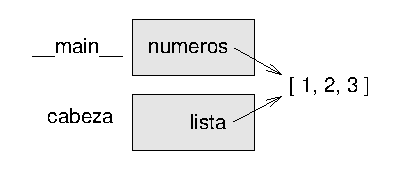
\includegraphics{illustrations/stack5.eps}}
\afterfig

Como el objeto lista está compartido por dos marcos, lo
dibujamos en el medio.

Si una función modifica un parámetro de tipo lista, el que hizo el llamado
ve los cambios. Por ejemplo, \texttt{borrarCabeza} borra el primer 
elemento de una lista:

\beforeverb
\begin{verbatim}
def borrarCabeza(lista):
  del lista[0]
\end{verbatim}
\afterverb
%
Y se puede usar así::

\beforeverb
\begin{verbatim}
>>> numeros = [1, 2, 3]
>>> borrarCabeza(numeros)
>>> print numeros
[2, 3]
\end{verbatim}
\afterverb
%
Si una función retorna una lista, retorna una referencia a ella.
Por ejemplo, la función \texttt{cola} retorna una lista que contiene 
todos los elementos, excepto el primero:

\beforeverb
\begin{verbatim}
def cola(lista):
  return lista[1:]
\end{verbatim}
\afterverb
%
\texttt{cola} se puede usar así:

\beforeverb
\begin{verbatim}
>>> numeros = [1, 2, 3]
>>> resto = cola(numeros)
>>> print resto
[2, 3]
\end{verbatim}
\afterverb
%
Como el valor de retorno se creó con el operador segmento, es una
nueva lista. La creación de  \texttt{resto}, y los cambios subsecuentes
sobre esta variable no tienen efecto sobre \texttt{numeros}.



\section{Listas anidadas}
\label{nested lists}
\index{listas anidadas}
\index{lista!anidada}

Una lista anidada aparece como elemento dentro de otra lista.
En la siguiente lista, el tercer elemento es una lista anidada:

\beforeverb
\begin{verbatim}
>>> lista = ["hola", 2.0, 5, [10, 20]]
\end{verbatim}
\afterverb
%
Si imprimimos \texttt{lista[3]}, vemos \texttt{[10, 20]}. Para 
tomar un elemento de la lista anidada podemos realizar dos pasos:

\beforeverb
\begin{verbatim}
>>> elt = lista[3]
>>> elt[0]
10
\end{verbatim}
\afterverb
%
O, los podemos combinar:

\beforeverb
\begin{verbatim}
>>> lista[3][1]
20
\end{verbatim}
\afterverb
%
Las aplicaciones del operador corchete se evalúan de izquierda a derecha, 
así que ésta expresión obtiene el elemento 3 de  \texttt{lista} y
extrae de allí el elemento 1.

\section{Matrices}
\index{matriz}
\index{lista!anidada}

Las listas anidadas se usan a menudo para representar matrices.  Por ejemplo,
la matriz:

\beforefig
\centerline{\includegraphics{illustrations/matrix.eps}}
\afterfig

se puede representar así:

\beforeverb
\begin{verbatim}
>>> matriz = [[1, 2, 3], [4, 5, 6], [7, 8, 9]]
\end{verbatim}
\afterverb
%
\texttt{matriz} es una lista con tres elementos, cada uno es una 
fila.  Podemos seleccionar una fila de la manera usual:

\beforeverb
\begin{verbatim}
>>> matriz[1]
[4, 5, 6]
\end{verbatim}
\afterverb
%
O podemos extraer un elemento individual de la matriz usando
dos índices:

\beforeverb
\begin{verbatim}
>>> matriz[1][1]
5
\end{verbatim}
\afterverb
%
El primero escoge la fila, y el segundo selecciona la columna.
Aunque esta forma de representar matrices es común, no es la
única posibilidad. Una pequeña variación consiste en usar una 
lista de columnas en lugar de una lista de filas. Más adelante
veremos una alternativa más radical, usando un diccionario.

\index{diccionario}
\index{fila}
\index{columna}


\section{Cadenas y listas}
\index{función split}
\index{función join}

Dos de las funciones más usadas del módulo  \texttt{string} implican
listas de cadenas. \texttt{split} separa una cadena en una lista
de palabras. Por defecto, cualquier número de espacios en blanco sirven
como criterio de separación:

\beforeverb
\begin{verbatim}
>>> import string
>>> cancion = "La vida es un ratico..."
>>> string.split(cancion)
['La', 'vida', 'es', 'un', 'ratico...']
\end{verbatim}
\afterverb
%
Un argumento opcional denominado  {\bf delimitador} se puede usar
para especificar que carácteres usar como criterio de separación.
El siguiente ejemplo usa la cadena \texttt{an} como delimitador:

\beforeverb
\begin{verbatim}
>>> string.split( "La rana que canta", "an")
['La r', 'a que c', 'ta']
\end{verbatim}
\afterverb
%
Note que el delimitador no aparece en la lista resultante.

La función \texttt{join} es la inversa de \texttt{split}.  Toma 
una lista de cadenas y las concatena con un espacio entre
cada par:

\beforeverb
\begin{verbatim}
>>> m = ['La', 'vida', 'es', 'un', 'ratico']
>>> string.join(m)
'La vida es un ratico'
\end{verbatim}
\afterverb
%
Como  \texttt{split}, \texttt{join} puede recibir un argumento 
adicional separador que se inserta entre los elementos:

\beforeverb
\begin{verbatim}
>>> string.join(m, '_')
'La_vida_es_un_ratico'
\end{verbatim}
\afterverb


\section{Glosario}

\begin{description}

\item[Lista:] colección de objetos que recibe un nombre. Cada objeto se
identifica con un índice o número entero positivo.

\item[Índice:] valor o variable entero que indica la posición de un elemento en una lista.

\item[Elemento:] uno de los valores dentro de una lista (u otra secuencia).  El 
operador corchete selecciona elementos de una lista.

\item[Secuencia:] los tipos de datos que contienen un conjunto ordenado de
elementos, identificados por índices.

\item[Lista anidada:] lista que es elemento de otra lista.

\item[Recorrido de una lista:] es el acceso secuencial de cada elemento de una lista.

\item[Objeto:] una cosa a la que una variable se puede referir.

\item[Alias:] cuando varias variables tienen referencias hacia el mismo objeto.

\item[Clonar:] crear un objeto con el mismo valor que un objeto preexistente.
Copiar una referencia a un objeto crea un alias, pero no clona el objeto.

\item[Delimitador:] carácter o cadena que se usa para indicar el lugar donde una cadena debe ser separada.

\index{lista}
\index{índice}
\index{secuencia}
\index{elemento}
\index{lista anidada}
\index{recorrido de una lista}
\index{objeto}
\index{alias}
\index{clonar}
\index{delimitador}

\end{description}

\section{Ejercicios}


Para cada función, agregue chequeo de tipos y pruebas unitarias.


\begin{enumerate}

 \item Escriba una función que  recorra una lista de cadenas 
   imprimiendo la longitud de cada una. ¿Qué pasa si usted
   le pasa un entero a  \texttt{len}?

 \item Describa la relación entre las expresiones: 
 
 \texttt{cadena} \hfill  {\tt string.join(string.split(cadena))}
 
 ¿Son iguales para todas las cadenas? 
 
 ¿Cuando serían diferentes?
  
  \item Escriba una función llamada \verb+esta_ordenada+ que tome una lista como parámetro y
  retorne True si la lista está ordenada de forma ascendente o False si no lo está.
  Usted puede asumir como precondición que los elementos son comparables con los 
  operadores relacionales. Por ejemplo: 
  
  \verb+esta_ordenada([1,2,2])+ debe retornar  True 
  
  \verb+esta_ordenada(['b','a'])+ debe retornar False.
  
  \item Dos palabras son anagramas si se pueden reordenar las letras de una palabra para formar
  la otra. Escriba una función llamada \verb+es_anagrama+ que tome dos cadenas y retorne True
  si son anagramas y False en caso contrario.
  
  \item Escriba una función llamada \verb+eliminar_duplicados+ que reciba una lista y retorne 
  una nueva lista con los elementos únicos de la original. No necesitan estar en el mismo 
  orden.
  
  
  \item Escriba dos versiones de una función que lea el archivo palabras.txt y construya una lista 
  con un elemento por palabra. Una versión usará el método append y la otra la construcción t=t+[x]. 
  ¿Cual es mas lenta? ¿Por qué?  Pista: use el módulo time para medir lo que tarda la ejecución 
  de las versiones.  
  
  palabras.txt: 
  http://cic.javerianacali.edu.co/~abecerra/files/palabras.txt
  
  Solución: 
  http://thinkpython.com/code/wordlist.py.

  \item Si hay un grupo de 23 personas, ¿cual es la probabilidad de que dos tengan la misma fecha
  de nacimiento?. Este valor puede estimarse generando muestras aleatorias de 23 cumpleaños y 
  contando las coincidencias. Pista: consulte la función randint del módulo random.
  
  Solución: 
  http://thinkpython.com/code/birthday.py
  
  \item Dos palabras son un "par inverso" si cada una es la inversa de la otra. Escriba un programa
  que encuentre todos los pares inversos del español (palabras.txt).
  
  \item Dos palabras se entretejen si tomando las letras de las dos, alternandose, se puede formar
  una nueva palabra. Por ejemplo: 'pie' y 'en' se entretejen en 'peine'.
  
  Solución: http://thinkpython.com/code/interlock.py
\end{enumerate}	\clearemptydoublepage  % listas
% LaTeX source for textbook ``How to think like a computer scientist'
% Copyright (c)  2001  Allen B. Downey, Jeffrey Elkner, and Chris Meyers.

% Permission is granted to copy, distribute and/or modify this
% document under the terms of the GNU Free Documentation License,
% Version 1.1  or any later version published by the Free Software
% Foundation; with the Invariant Sections being "Contributor List",
% with no Front-Cover Texts, and with no Back-Cover Texts. A copy of
% the license is included in the section entitled "GNU Free
% Documentation License".

% This distribution includes a file named fdl.tex that contains the text
% of the GNU Free Documentation License.  If it is missing, you can obtain
% it from www.gnu.org or by writing to the Free Software Foundation,
% Inc., 59 Temple Place - Suite 330, Boston, MA 02111-1307, USA.



\chapter{Tuplas}
\label{tuplechap}
\index{tupla}

\section{Mutabilidad y tuplas}
\index{tupla}
\index{tipo de dato!tupla}
\index{tipo de dato!inmutable}

Hasta aquí, usted ha visto dos tipos de datos compuestos: cadenas, que están
compuestas de carácteres; y listas, compuestas de elementos de
cualquier tipo. Una de las diferencias que notamos es que los elementos
de una lista pueden modificarse, pero los carácteres en una cadena no.
En otras palabras, las cadenas son {\bf inmutables} y las listas 
son {\bf mutables}.

\index{mutable}
\index{inmutable}

Hay otro tipo de dato en Python denominado {\bf tupla}, que se parece a una 
lista, con la excepción de que es inmutable.  Sintácticamente, una tupla es 
una lista de valores separados por comas:

\beforeverb
\begin{verbatim}
>>> tupla = 'a', 'b', 'c', 'd', 'e'
\end{verbatim}
\afterverb
%
Aunque no es necesario, se pueden encerrar entre paréntesis:

\beforeverb
\begin{verbatim}
>>> tupla = ('a', 'b', 'c', 'd', 'e')
\end{verbatim}
\afterverb
%
Para crear una tupla con un único elemento, tenemos que incluir
la coma final:

\beforeverb
\begin{verbatim}
>>> t1 = ('a',)
>>> type(t1)
<type 'tuple'>
\end{verbatim}
\afterverb
%
Sin la coma, Python creería que  \texttt{('a')} es una cadena en
paréntesis:

\beforeverb
\begin{verbatim}
>>> t2 = ('a')
>>> type(t2)
<type 'string'>
\end{verbatim}
\afterverb
%
Las operaciones sobre tuplas son las mismas que vimos con las
listas. El operador corchete selecciona un elemento de la 
tupla.

\beforeverb
\begin{verbatim}
>>> tupla = ('a', 'b', 'c', 'd', 'e')
>>> tupla[0]
'a'
\end{verbatim}
\afterverb
%
Y el operador segmento selecciona un rango de elementos:

\beforeverb
\begin{verbatim}
>>> tupla[1:3]
('b', 'c')
\end{verbatim}
\afterverb
%
Pero si intentamos modificar un elemento de la tupla obtenemos un
error:

\index{error en tiempo de ejecución}

\beforeverb
\begin{verbatim}
>>> tupla[0] = 'A'
TypeError: object doesn't support item assignment
\end{verbatim}
\afterverb
%
Aunque no podemos modificar los elementos, sí
podemos modificar toda la tupla:

\beforeverb
\begin{verbatim}
>>> tupla = ('A',) + tupla[1:]
>>> tupla
('A', 'b', 'c', 'd', 'e')
>>> tupla = (1,2,3)
>>> tupla
\end{verbatim}
\afterverb
%

\section{Asignación de tuplas}
\label{tuple assignment}
\index{asignación de tuplas}
\index{Asignación!de tuplas}

De vez en cuando necesitamos intercambiar los valores de dos variables.
Con el operador de  asignación normal tenemos que usar una variable
temporal.  Por ejemplo, para intercambiar \texttt{a} y \texttt{b}:

\beforeverb
\begin{verbatim}
>>> temp = a
>>> a = b
>>> b = temp
\end{verbatim}
\afterverb
%
Si tenemos que intercambiar variables muchas veces, el código tiende
a ser engorroso. Python proporciona una forma de {\bf asignación de tuplas} que
resuelve este problema:

\beforeverb
\begin{verbatim}
>>> a, b = b, a
\end{verbatim}
\afterverb
%
El lado izquierdo es una tupla de variables; el derecho es una tupla
de valores. Cada valor se asigna a su respectiva variable en el orden 
en que se presenta. Las expresiones en el lado derecho se evalúan
antes de cualquier asignación. Esto hace a la asignación de tuplas
una herramienta bastante versátil.

Naturalmente, el número de variables a la izquierda y el número de
valores a la derecha deben coincidir.

\beforeverb
\begin{verbatim}
>>> a, b, c, d = 1, 2, 3
ValueError: unpack tuple of wrong size
\end{verbatim}
\afterverb
%

\section{Tuplas como valores de retorno}
\index{tupla}
\index{valor!tupla}
\index{valor de retorno!tupla}
\index{función!tupla como valor de retorno}

Las funciones pueden tener tuplas como valores de retorno. Por
ejemplo, podríamos escribir una función que intercambie sus
dos parámetros:

\beforeverb
\begin{verbatim}
def intercambiar(x, y):
  return y, x
\end{verbatim}
\afterverb
%
Así podemos asignar el valor de retorno a una tupla con dos variables:

\beforeverb
\begin{verbatim}
a, b = intercambiar(a, b)
\end{verbatim}
\afterverb
%
En este caso, escribir una función  \texttt{intercambio} no es muy 
provechoso. De hecho, hay un peligro al tratar de encapsular {\tt
intercambio}, que consiste en el siguiente error:

\beforeverb
\begin{verbatim}
def intercambio(x, y):      # version incorrecta
  x, y = y, x
\end{verbatim}
\afterverb
%
Si llamamos a esta función así:

\beforeverb
\begin{verbatim}
intercambio(a, b)
\end{verbatim}
\afterverb
%
entonces \texttt{a} y \texttt{x} son dos alias para el mismo valor.  Cambiar \texttt{x}
dentro de \texttt{intercambio} hace que  \texttt{x} se refiera a un valor diferente, 
pero no tiene efecto en la \texttt{a} dentro de  \texttt{\_\_main\_\_}.  Igualmente, 
cambiar \texttt{y} no tiene efecto en  \texttt{b}.

Esta función se ejecuta sin errores, pero no hace lo que se pretende.
Es un ejemplo de error semántico.

\index{error semántico}




\section{Números aleatorios}
\index{número aleatorio}
\index{número!aleatorio}

La gran mayoría de los programas hacen lo mismo cada vez que se ejecutan,
esto es, son  {\bf determinísticos}.  El determinismo generalmente es 
una buena propiedad, ya que usualmente esperamos que los cálculos
produzcan el mismo resultado. Sin embargo, para algunas aplicaciones
necesitamos que el computador sea impredecible. Los juegos son un 
ejemplo inmediato, pero hay más.

Lograr que un programa sea verdaderamente no determinístico no es una
tarea fácil, pero hay formas de que parezca no determinístico. Una
de ellas es generar números aleatorios y usarlos para determinar
la salida de un programa. Python tiene una función primitiva
que genera números {\bf pseudoaleatorios}, que, aunque no sean
aleatorios desde el punto de vista matemático, sirven para nuestros
propósitos.

El módulo  \texttt{random} contiene una función llamada \texttt{random} que
retorna un número flotante entre 0.0 y 1.0.  Cada vez que se llama a
\texttt{random}, se obtiene el siguiente número de una serie muy larga.
Para ver un ejemplo ejecute el siguiente ciclo:

\beforeverb
\begin{verbatim}
import random

for i in range(10):
  x = random.random()
  print x
\end{verbatim}
\afterverb
%
Para generar un número aleatorio entre 0.0 y un límite superior
como \texttt{sup}, multiplique \texttt{x} por \texttt{sup}.



\section{Lista de números aleatorios}

Vamos a generar función que cree una lista de números aleatorios \texttt{listaAleatoria},
recibirá un parámetro entero que especifique el número de elementos a generar.
Primero, genera una lista de  \texttt{n} ceros. Luego cada vez que itera 
en un ciclo for, reemplaza uno de los ceros por un número aleatorio.
El valor de retorno es una referencia a la lista construida:

\beforeverb
\begin{verbatim}
def listaAleatoria(n):
  s = [0] * n
  for i in range(n):
    s[i] = random.random()
  return s
\end{verbatim}
\afterverb
%
La probaremos con ocho elementos. Para depurar es una buena
idea empezar con pocos datos:

\adjustpage{-2}
\beforeverb
\begin{verbatim}
>>> listaAleatoria(8)
0.15156642489
0.498048560109
0.810894847068
0.360371157682
0.275119183077
0.328578797631
0.759199803101
0.800367163582
\end{verbatim}
\afterverb
%
Los números generados por \texttt{random} deben distribuirse uniformemente,
lo que significa que cada valor es igualmente probable.

Si dividimos el rango de  valores posibles en ``regiones'' del mismo
tamaño y contamos el número de veces que un valor aleatorio cae
en cada región, deberíamos obtener un resultado aproximado en todas
las regiones.

Podemos probar esta hipótesis escribiendo un programa que
divida el rango en regiones y cuente el número de valores que caen
en cada una.


\section{Conteo}
\index{conteo}

Un enfoque que funciona en problemas como éste es dividir el problema
en subproblemas que se puedan resolver con un patrón computacional
que ya sepamos.

En este caso, necesitamos recorrer una lista de números y contar
el número de veces que un valor cae en un rango dado. Esto parece
familiar. En la Sección~\ref{counter}, escribimos un programa
que recorría una cadena y contaba el números de veces que aparecía
una letra determinada.

Entonces podemos copiar el programa viejo para adaptarlo posteriormente
a nuestro problema actual. El original es:

\beforeverb
\begin{verbatim}
cont = 0
for c in fruta:
  if c == 'a':
    cont = cont + 1
print cont
\end{verbatim}
\afterverb
%
El primer paso es reemplazar  \texttt{fruta} con \texttt{lista} y 
\texttt{c} por \texttt{num}.  Esto no cambia el programa, sólo lo hace
más legible.

El segundo paso es cambiar la prueba. No queremos buscar letras.
Queremos ver si  \texttt{num} está entre dos valores dados
\texttt{inf} y  \texttt{sup}.

\beforeverb
\begin{verbatim}
cont = 0
for num in lista:
  if inf < num < sup:
    cont = cont + 1
print cont
\end{verbatim}
\afterverb
%
El último paso consiste en  encapsular este código en una
función denominada \texttt{enRegion}.  Los parámetros son la lista
y los valores \texttt{inf} y \texttt{sup}.

\beforeverb
\begin{verbatim}
def enRegion(lista, inf, sup):
  cont = 0
  for num in lista:
    if inf < num < sup:
      cont = cont + 1
  return cont
\end{verbatim}
\afterverb
%
Copiando y modificando un programa existente fuimos capaces
de escribir esta función rápidamente y ahorrarnos un buen
tiempo de depuración. Este plan de desarrollo se denomina
{\bf concordancia de patrones}. Si se encuentra trabajando 
en un problema que ya ha resuelto antes, reutilice la 
solución.

\section{Muchas regiones}
\label{muchasregiones}

Como el número de regiones aumenta, \texttt{enRegion} es 
un poco engorroso. Con dos no esta tan mal:

\beforeverb
\begin{verbatim}
inf = enRegion(a, 0.0, 0.5)
sup = enRegion(a, 0.5, 1)
\end{verbatim}
\afterverb
%
Pero con cuatro:

\beforeverb
\begin{verbatim}
Region1 = enRegion(a, 0.0, 0.25)
Region2 = enRegion(a, 0.25, 0.5)
Region3 = enRegion(a, 0.5, 0.75)
Region4 = enRegion(a, 0.75, 1.0)
\end{verbatim}
\afterverb
%
Hay dos problemas. Uno es que siempre tenemos que crear
nuevos nombres de variables para cada resultado. El otro
es que tenemos que calcular el rango de cada región.

Primero resolveremos el segundo problema. Si el número de
regiones está dado por la variable \texttt{numRegiones}, entonces, 
el ancho de cada región está dado por la expresión \texttt{1.0/numRegiones}.

Usaremos un ciclo para calcular el rango de cada región.
La variable de ciclo \texttt{i} cuenta de 1 a \texttt{numRegiones-1}:

\beforeverb
\begin{verbatim}
ancho = 1.0 / numRegiones
for i in range(numRegiones):
  inf = i * ancho
  sup = inf + ancho
  print inf, " hasta ", sup
\end{verbatim}
\afterverb
%
Para calcular el extremo inferior de cada región, multiplicamos
la variable de ciclo por el ancho. El extremo superior está
 a un  \texttt{ancho} de región de distancia.

Con \texttt{numRegiones = 8}, la salida es:

\beforeverb
\begin{verbatim}
0.0 hasta 0.125
0.125 hasta 0.25
0.25 hasta 0.375
0.375 hasta 0.5
0.5 hasta 0.625
0.625 hasta 0.75
0.75 hasta 0.875
0.875 hasta 1.0
\end{verbatim}
\afterverb
%
Usted puede confirmar que cada región tiene el mismo ancho,
que no se solapan y que cubren el rango completo de  0.0 a 1.0.

Ahora regresemos al primer problema. Necesitamos una manera
de almacenar ocho enteros, usando una variable para indicarlos
uno a uno.  Usted debe estar pensando ``¡una lista!''

Tenemos que crear la lista de regiones fuera del ciclo, porque 
esto sólo debe ocurrir una vez. Dentro del ciclo, llamaremos
a \texttt{enRegion} repetidamente y actualizaremos el  \texttt{i}ésimo 
elemento de la lista:

\beforeverb
\begin{verbatim}
numRegiones = 8
Regiones = [0] * numRegiones
ancho = 1.0 / numRegiones
for i in range(numRegiones):
  inf = i * ancho
  sup = inf + ancho
  Regiones[i] = enRegion(lista, inf, sup)
print Regiones
\end{verbatim}
\afterverb
%
Con una lista de 1000 valores, este código produce la siguiente lista
de conteo:

\beforeverb
\begin{verbatim}
[138, 124, 128, 118, 130, 117, 114, 131]
\end{verbatim}
\afterverb
%
Todos estos valores están muy cerca a 125, que es lo que esperamos.
Al menos, están lo suficientemente cerca como para creer que el
generador de números pseudoaleatorios está funcionando bien.




\section{Una solución en una sola pasada}
\label{histograma}
\index{histograma}

Aunque funciona, este programa no es tan eficiente como debería.
Cada vez que llama a \texttt{enRegion}, recorre la lista entera.  A medida
que el número de regiones incrementa, va a hacer muchos
recorridos.

Sería mejor hacer una sola pasada a través de la lista y calcular
para cada región el índice de la región en la que cae. Así podemos
incrementar el contador apropiado.

En la sección anterior tomamos un índice \texttt{i} y lo multiplicamos
por el \texttt{ancho} para encontrar el extremo inferior de una región. 
Ahora vamos a encontrar el índice de la región en la que cae.

Como este problema es el inverso del anterior, podemos intentar
dividir por \texttt{ancho} en vez de multiplicar. ¡Esto funciona!

Como \texttt{ancho = 1.0 / numRegiones}, dividir por {\tt
ancho} es lo mismo que multiplicar por \texttt{numRegiones}.  Si 
multiplicamos un número en el rango 0.0 a 1.0 por \texttt{numRegiones}, 
obtenemos un número en el rango de  0.0 a \texttt{numRegiones}.  Si 
redondeamos ese número al entero más cercano por debajo, obtenemos
lo que queremos: un índice de región:

\beforeverb
\begin{verbatim}
numRegiones = 8
Regiones = [0] * numRegiones
for i in lista:
  ind = int(i * numRegiones)
  Regiones[ind] = Regiones[ind] + 1
\end{verbatim}
\afterverb
%
Usamos la función  \texttt{int} para pasar de número de punto flotante
a entero.

¿Es posible que este programa produzca un índice que esté fuera
de rango (por ser negativo o mayor que \texttt{len(Regiones)-1})?

Una lista como  \texttt{Regiones} que almacena los conteos del número
de valores que hay en cada rango se denomina {\bf histograma}.



\section{Glosario}

\begin{description}

\item[Tipo inmutable:] es un tipo de dato en el que los elementos no
pueden ser modificados. Las asignaciones a elementos o segmentos
de tipos inmutables causan errores. Las cadenas y las tuplas son
inmutables.

\item[Tipo mutable:] tipo de dato en el que los elementos 
pueden ser modificados. Todos los tipos mutables son compuestos.
Las listas y los diccionarios son mutables.

\item[Tupla:] tipo de dato secuencial similar a la lista, pero 
inmutable.  Las tuplas se pueden usar donde se requiera un tipo inmutable,
por ejemplo como llaves de un diccionario.

\item[Asignación de tuplas:] una asignación a todos los elementos de una tupla
en una sola sentencia. La asignación ocurre en paralelo y no secuencialmente.
Es útil para intercambiar valores de variables.

\item[Determinístico:] programa que hace lo mismo cada vez que se llama.

\item[Pseudoaleatoria:] secuencia de números que parece aleatoria, pero
en realidad es el resultado de un cómputo determinístico, bien diseñado.

\item[Histograma:]  lista de enteros en la que cada elemento cuenta
el número de veces que algo sucede.

\item[Correspondencia de patrones:] plan de desarrollo de programas que
implica identificar un patrón computacional familiar y copiar la 
solución de un problema similar.

\index{tipo mutable}
\index{tipo inmutable}
\index{tupla}
\index{asignación de tupla}
\index{asignación!de tupla}
\index{determinístic}
\index{pseudoaleatorio}
\index{histograma}
\index{correspondencia de patrones}

\end{description}

\section{Ejercicios}


Para cada función, agregue chequeo de tipos y pruebas unitarias.


\begin{enumerate}

 \item Escriba una función mas\_frecuentes que tome una cadena e imprima las letras en orden descendente por frecuencia.
 Ejecutela con textos de diferentes lenguajes y observe como varían las frecuencias de letras. Compare sus resultados
 con las tablas en:
 
 http://en.wikipedia.org/wiki/Letter\_frequencies. 
 
 Solución: http://thinkpython.com/code/most\_frequent.py. 
  
 \item Escriba un programa que lea una lista de palabras de un archivos e imprima todos los conjuntos de palabras que 
 son anagramas.
 
 Este es un ejemplo con palabras en inglés de la salida del programa:

 ['deltas', 'desalt', 'lasted', 'salted', 'slated', 'staled']
 ['retainers', 'ternaries']
 ['generating', 'greatening']
 ['resmelts', 'smelters', 'termless']

 Pista: cree un diccionario que asocie cada conjunto de letras a una lista de palabras que puedan ser formadas con 
 esas letras. ¿Como se puede representar el conjunto de letras de forma que pueda ser usado como llave?
 Modifique el programa que obtuvo para que imprima en orden descendente por tamaño los conjuntos de anagramas.
 En el juego Scrabble, un 'bingo' se da cuando se juegan las 7 fichas, junto con otra letra en el tablero, para formar
 una palabra de 8 letras. ¿Que conjunto de 8 letras forma los bingos mas posibles? 
 
 
 Solución: http://thinkpython.com/code/anagram\_sets.py.

 \item Dos palabras forma un 'par de metatesis' si se puede transformar una en otra intercambiando dos letras. Por ejemplo,
 'conversación' y 'conservación'. Escriba un programa que encuentre todos los pares de metatesis en el diccionario. Pista: 
 no pruebe todos los pares.
 
 Solución: http://thinkpython.com/code/metathesis.py. 
 
 Crédito: el ejercicio está inspirado por un ejemplo en http://puzzlers.org.

 
 \item
 ¿Cual es la palabra mas larga que sigue siendo válida a medida que se remueven una a una sus letras?
 Por ejemplo, en inglés, 'sprite' sin la 'r' es 'spite', que sin la 'e', es 'spit', que sin la 's' es
 'pit', que sin la 'p' es 'it' que sin la 't' es 'i'. Las letras se pueden remover de cualquier posición, pero no se 
 pueden reordenar.
 
 Escriba un programa que encuentre todas las palabras que pueden reducirse de esta forma y que encuentre la mas larga.

 Pistas:
 
 Escriba una función que tome una palabra y calcule todas las palabras que pueden formarse al removerle una letra. Estas
 son las palabras 'hijas'.
 Recursivamente, una palabra es reducible si alguno de sus hijas es reducible. El caso base lo da la cadena vacía.
  
 Solución: http://thinkpython.com/code/reducible.py.
\end{enumerate}
	\clearemptydoublepage  % tuplas
% LaTeX source for textbook ``How to think like a computer scientist''
% Copyright (c)  2001  Allen B. Downey, Jeffrey Elkner, and Chris Meyers.

% Permission is granted to copy, distribute and/or modify this
% document under the terms of the GNU Free Documentation License,
% Version 1.1  or any later version published by the Free Software
% Foundation; with the Invariant Sections being "Contributor List",
% with no Front-Cover Texts, and with no Back-Cover Texts. A copy of
% the license is included in the section entitled "GNU Free
% Documentation License".

% This distribution includes a file named fdl.tex that contains the text
% of the GNU Free Documentation License.  If it is missing, you can obtain
% it from www.gnu.org or by writing to the Free Software Foundation,
% Inc., 59 Temple Place - Suite 330, Boston, MA 02111-1307, USA.

\chapter{Diccionarios}

\index{diccionarios}
\index{diccionario}
\index{tipo de datos!diccionario}
\index{clave}
\index{par clave-valor}
\index{índice}

Los tipos compuestos que ha visto hasta ahora (cadenas, listas y tuplas) usan enteros como índices. 
Si usted intenta usar cualquier otro tipo como índice provocará un error.

Los {\bf diccionarios} son similares a otros tipos compuestos, excepto en que pueden usar 
como índice cualquier tipo inmutable. A modo de ejemplo, crearemos un diccionario que traduzca 
palabras inglesas al español. En este diccionario, los índices son cadenas \texttt{(strings)}.

Una forma de crear un diccionario es empezar con el diccionario vacío y añadir elementos. El 
diccionario vacío se expresa como \texttt{\{\}}:

\beforeverb
\begin{verbatim}
>>> ing_a_esp = {}
>>> ing_a_esp['one'] = 'uno'
>>> ing_a_esp['two'] = 'dos'
\end{verbatim}
\afterverb
%
La primera asignación crea un diccionario llamado \texttt{ing\_a\_esp}; las otras asignaciones 
añaden nuevos elementos al diccionario. Podemos desplegar el valor actual del diccionario 
del modo habitual:

\beforeverb
\begin{verbatim}
>>> print ing_a_esp
{'one': 'uno', 'two': 'dos'}
\end{verbatim}
\afterverb
%
Los elementos de un diccionario aparecen en una lista separada por comas. Cada entrada 
contiene un índice y un valor separado por dos puntos (:). En un diccionario, los índices 
se llaman {\bf claves}, por eso los elementos se llaman {\bf pares clave-valor}.

Otra forma de crear un diccionario es dando una lista de pares clave-valor con la misma 
sintaxis que la salida del ejemplo anterior:

\beforeverb
\begin{verbatim}
>>> ing_a_esp={'one': 'uno', 'two': 'dos', 'three': 'tres'}
\end{verbatim}
\afterverb
%
Si volvemos a imprimir el valor de \texttt{ing\_a\_esp}, nos llevamos una sorpresa:

\beforeverb
\begin{verbatim}
>>> print ing_a_esp
{'one': 'uno', 'three': 'tres', 'two': 'dos'}
\end{verbatim}
\afterverb
%
¡Los pares clave-valor no están en orden! Afortunadamente, no necesitamos preocuparnos 
por el orden, ya que los elementos de un diccionario nunca se indexan con índices enteros. 
En lugar de eso, usamos las claves para buscar los valores correspondientes:

\beforeverb
\begin{verbatim}
>>> print ing_a_esp['two']
'dos'
\end{verbatim}
\afterverb
%
La clave \texttt{'two'} nos da el valor \texttt{'dos'} aunque aparezca en el 
tercer par clave-valor.


\section{Operaciones sobre diccionarios}
\index{diccionario!operaciones}
\index{diccionarios!operaciones sobre}

La sentencia \texttt{del} elimina un par clave-valor de un diccionario. Por ejemplo, 
el diccionario siguiente contiene los nombres de varias frutas y el número de esas 
frutas en un almacén:

\beforeverb
\begin{verbatim}
>>> inventario = {'manzanas': 430, 'bananas': 312, 
       'naranjas': 525,   'peras': 217}
>>> print inventario
{'naranjas': 525, 'manzanas': 430, 'peras': 217, 
 'bananas': 312}
\end{verbatim}
\afterverb
%
Si alguien compra todas las peras, podemos eliminar la entrada del diccionario:

\beforeverb
\begin{verbatim}
>>> del inventario['peras']
>>> print inventario
{'naranjas': 525, 'manzanas': 430, 'bananas': 312}
\end{verbatim}
\afterverb
%
O si esperamos recibir más peras pronto, podemos simplemente cambiar el inventario asociado con las peras:

\beforeverb
\begin{verbatim}
>>> inventario['peras'] = 0
>>> print inventario
{'naranjas': 525, 'manzanas': 430, 'peras': 0, 
 'bananas': 312}
\end{verbatim}
\afterverb
%
La función \texttt{len} también funciona con diccionarios; devuelve el número de pares clave-valor:

\beforeverb
\begin{verbatim}
>>> len(inventario)
4
\end{verbatim}
\afterverb
%


\section{Métodos del diccionario}
\index{diccionario!métodos}
\index{método}
\index{método!invocación}
\index{diccionarios!métodos}
\index{métodos sobre diccionarios}
\index{invocar métodos}

Un {\bf método} es similar a una función, acepta parámetros y devuelve un valor, 
pero la sintaxis es diferente. Por ejemplo, el método \texttt{keys} acepta un 
diccionario y devuelve una lista con las claves que aparecen, pero en lugar de 
la sintaxis de llamado de función \texttt{keys(ing\_a\_esp)}, usamos la 
sintaxis para un método \texttt{ing\_a\_esp.keys()}.

\index{notación de punto}

\beforeverb
\begin{verbatim}
>>> ing_a_esp.keys()
['one', 'three', 'two']
\end{verbatim}
\afterverb
%
Esta forma de notación punto especifica el nombre de la función, \texttt{keys}, 
y el nombre del objeto al que se va a aplicar la función, \texttt{ing\_a\_esp}. 
Los paréntesis indican que este método no admite parámetros.

La llamada a un método se denomina {\bf invocación}; en este caso, diríamos 
que estamos invocando \texttt{keys} sobre el objeto \texttt{ing\_a\_esp}.

El método \texttt{values} es similar; devuelve una lista de los valores del 
diccionario:

\beforeverb
\begin{verbatim}
>>> ing_a_esp.values()
['uno', 'tres', 'dos']
\end{verbatim}
\afterverb
%
El método \texttt{items} devuelve ambos, una lista de tuplas con los pares 
clave-valor del diccionario:

\beforeverb
\begin{verbatim}
>>> ing_a_esp.items()
[('one','uno'), ('three', 'tres'), ('two', 'dos')]
\end{verbatim}
\afterverb
%
La sintaxis nos proporciona información muy útil acerca del tipo de datos. 
Los corchetes indican que es una lista. Los paréntesis indican que los 
elementos de la lista son tuplas.

Si un método acepta un argumento, usa la misma sintaxis que una 
llamada a una función. Por ejemplo, el método \texttt{has\_key} acepta 
una clave y devuelve verdadero (1) si la clave aparece en el diccionario:

\beforeverb
\begin{verbatim}
>>> ing_a_esp.has_key('one')
True
>>> ing_a_esp.has_key('deux')
False
\end{verbatim}
\afterverb
%
Si se invoca un método sin especificar un objeto, se genera 
un error. En este caso, el mensaje de error no es de mucha ayuda:

\beforeverb
\begin{verbatim}
>>> has_key('one')
NameError: has_key
\end{verbatim}
\afterverb
%

\index{error en tiempo de ejecución}


\section{Copiado y alias}
\index{asignación de alias}
\index{copiado}
\index{clonado}

Usted debe estar atento a los alias debido a la mutabilidad de los diccionarios. Si dos variables se refieren al mismo objeto los cambios en una afectan a la otra.

Si quiere modificar un diccionario y mantener una copia del original, se
puede usar el método \texttt{copy}. Por ejemplo, \texttt{opuestos} es un diccionario que contiene pares de opuestos:

\beforeverb
\begin{verbatim}
>>> opuestos = {'arriba': 'abajo', 'derecho': 'torcido', 
  'verdadero': 'falso'}
>>> alias = opuestos
>>> copia = opuestos.copy()
\end{verbatim}
\afterverb
%
\texttt{alias} y \texttt{opuestos} se refieren al mismo objeto; \texttt{copia} se refiere a una copia nueva del mismo diccionario. Si modificamos \texttt{alias}, \texttt{opuestos} también resulta cambiado:

\beforeverb
\begin{verbatim}
>>> alias['derecho'] = 'sentado'
>>> opuestos['derecho']
'sentado'
\end{verbatim}
\afterverb
%
Si modificamos \texttt{copia}, \texttt{opuestos} no varía:

\beforeverb
\begin{verbatim}
>>> copia['derecho'] = 'privilegio'
>>> opuestos['derecho']
'sentado'
\end{verbatim}
\afterverb
%


\section{Matrices dispersas}
\index{matriz!dispersa}
\index{lista anidada}
\index{lista!anidada}

En la Sección~\ref{nested lists} usamos una lista de listas para representar una matriz. 
Es una buena opción para una matriz en la que la mayoría de los valores es diferente de cero, 
pero piense en una matriz como ésta:

%\beforefig
\centerline{\includegraphics{illustrations/sparse.eps}}
%\afterfig

La representación de la lista contiene un montón de ceros:

%\pagebreak
%\beforeverb
\begin{verbatim}
>>> matriz = [ [0,0,0,1,0],
           [0,0,0,0,0],
           [0,2,0,0,0],
           [0,0,0,0,0],
           [0,0,0,3,0] ]
\end{verbatim}
%\afterverb
%
Una posible alternativa consiste en usar un diccionario. Como claves, podemos usar tuplas que contengan los números de fila y columna. Ésta es la representación de la misma matriz por medio de un diccionario:

%\beforeverb
\begin{verbatim}
>>> matriz = {(0,3): 1, (2, 1): 2, (4, 3): 3}
\end{verbatim}
%\afterverb
%
Sólo hay tres pares clave-valor, uno para cada elemento de la matriz diferente de cero. Cada clave es una tupla, y cada valor es un entero.

Para acceder a un elemento de la matriz, podemos usar el operador \texttt{[]}:

\beforeverb
\begin{verbatim}
>>> matriz[0,3]
1
\end{verbatim}
\afterverb
%
Observe que la sintaxis para la representación por medio del diccionario no es la misma de la representación por medio de la lista anidada. En lugar de dos índices enteros, usamos un índice compuesto que es una tupla de enteros.

Hay un problema. Si apuntamos a un elemento que es cero, se produce un error porque en el diccionario no hay una entrada con esa clave:

\index{error en tiempo de ejecución}

\beforeverb
\begin{verbatim}
>>> matriz[1,3]
KeyError: (1, 3)
\end{verbatim}
\afterverb
%
El método \texttt{get} soluciona este problema:

\beforeverb
\begin{verbatim}
>>> matriz.get((0,3), 0)
1
\end{verbatim}
\afterverb
%
El primer argumento es la clave; el segundo argumento es el valor que debe devolver \texttt{get} en caso de que la clave no esté en el diccionario:

\beforeverb
\begin{verbatim}
>>> matriz.get((1,3), 0)
0
\end{verbatim}
\afterverb
%
\texttt{get} mejora sensiblemente la semántica del acceso a una matriz dispersa. ¡Lástima que la  sintaxis no sea tan clara!


\section{Pistas}
\index{pista}
\index{función de Fibonacci}

Si ha jugado con la función \texttt{fibonacci} de la Sección~\ref{one more example}, es posible que haya notado que cuanto más grande es el argumento que recibe, más tiempo le cuesta ejecutarse. De hecho, el tiempo de ejecución aumenta muy rápidamente. En nuestra máquina, \texttt{fibonacci(20)} acaba instantáneamente, \texttt{fibonacci(30)} tarda más o menos un segundo, y \texttt{fibonacci(40)} tarda una eternidad.

Para entender por qué, observe este {\bf gráfico de llamadas} de \texttt{fibonacci} con \texttt{n=4}:

\beforefig
\centerline{\includegraphics{illustrations/fibonacci.eps}}
\afterfig

Un gráfico de llamadas muestra un conjunto de cajas de función con líneas que conectan cada caja con las cajas de las funciones a las que llama. En lo alto del gráfico, \texttt{fibonacci} con \texttt{n=4} llama a \texttt{fibonacci} con \texttt{n=3} y \texttt{n=2}. A su vez, \texttt{fibonacci} con \texttt{n=3} llama a \texttt{fibonacci} con \texttt{n=2} y \texttt{n=1}. Y así sucesivamente.

\index{caja de función}
\index{caja}
\index{gráfico de llamadas}

Cuente cuántas veces se llama a \texttt{fibonacci(0)} y \texttt{fibonacci(1)}. Esta función es una solución ineficiente para
el problema, y empeora mucho a medida que crece el argumento.

Una buena solución es llevar un registro de los valores que ya se 
han calculado almacenándolos en un diccionario. A un valor que ya 
ha sido calculado y almacenado para un uso posterior se le llama 
{\bf pista}. Aquí hay una implementación de \texttt{fibonacci} con pistas:

\beforeverb
\begin{verbatim}
anteriores = {0:1, 1:1}

def fibonacci(n):
  if anteriores.has_key(n):
    return anteriores[n]
  else:
    nuevoValor = fibonacci(n-1) + fibonacci(n-2)
    anteriores[n] = nuevoValor
    return nuevoValor
\end{verbatim}
\afterverb
%
El diccionario llamado \texttt{anteriores} mantiene un registro de 
los valores de Fibonacci que ya conocemos. El programa comienza con 
sólo dos pares: 0 corresponde a 1 y 1 corresponde a 1.

Siempre que se llama a \texttt{fibonacci} comprueba si el diccionario 
contiene el resultado ya calculado.  Si está ahí, la función puede 
devolver el valor inmediatamente sin hacer más llamadas recursivas. 
Si no, tiene que calcular el nuevo valor. El nuevo valor se añade 
al diccionario antes de que la función retorne.

Con esta versión de \texttt{fibonacci}, nuestra máquina puede calcular 
\texttt{fibonacci(40)} en un abrir y cerrar de ojos. Pero cuando 
intentamos calcular \texttt{fibonacci(50)}, nos encontramos con otro 
problema:

\index{error en tiempo de ejecución}
\index{desbordamiento}

\beforeverb
\begin{verbatim}
>>> fibonacci(50)
OverflowError: integer addition
\end{verbatim}
\afterverb
%
La respuesta, como se verá en un momento, es 20.365.011.074.  El problema es que este número es demasiado grande para caber en un entero de Python. Se {\bf desborda}. Afortunadamente, hay una solución fácil para este problema.


\section{Enteros largos}
\index{enteros largos}
\index{tipos de datos!enteros largos}
\index{enteros!largos}

Python proporciona un tipo llamado \texttt{long int} que puede manejar enteros de cualquier tamaño. Hay dos formas de crear un valor \texttt{long int}. Una es escribir un entero con una {\em L} mayúscula al final:

\beforeverb
\begin{verbatim}
>>> type(1L)
<type 'long int'>
\end{verbatim}
\afterverb
%
La otra es usar la función \texttt{long} para convertir un valor en \texttt{long int}. \texttt{long} acepta cualquier tipo numérico e incluso cadenas de dígitos:

\beforeverb
\begin{verbatim}
>>> long(1)
1L
>>> long(3.9)
3L
>>> long('57')
57L
\end{verbatim}
\afterverb
%
Todas las operaciones matemáticas funcionan sobre los datos de tipo \texttt{long int}, 
así que no tenemos que hacer mucho para adaptar \texttt{fibonacci}:

\beforeverb
\begin{verbatim}
>>> anterior = {0:1L, 1:1L}
>>> fibonacci(50)
20365011074L
\end{verbatim}
\afterverb
%
Simplemente cambiando el contenido inicial de \texttt{anteriores} cambiamos el comportamiento de \texttt{fibonacci}. Los primeros dos números de la secuencia son de tipo  \texttt{long int}, así que todos los números subsiguientes lo serán también.

\index{forzado de tipo de datos}
\index{coerción!tipo}

\begin{quote}
{\em Como ejercicio, modifica \texttt{factorial} de forma que produzca un \texttt{long int} como resultado.}
\end{quote}


\section{Contar letras}
\index{recuento}
\index{histograma}
\index{compresión}

En el capítulo~\ref{strings} escribimos una función que contaba el número de apariciones de una letra en una cadena. Una versión más genérica de este problema es crear un histograma de las letras de la cadena, o sea, cuántas veces aparece cada letra.

Ese histograma podría ser útil para comprimir un archivo de texto. Como las diferentes letras aparecen con frecuencias distintas, podemos comprimir un archivo usando códigos cortos para las letras más habituales y códigos más largos para las que aparecen con menor frecuencia.

Los diccionarios facilitan una forma elegante de generar un histograma:

\beforeverb
\begin{verbatim}
>>> cuentaLetras = {}
>>> for letra in "Mississippi":
...   cuentaLetras[letra] = cuentaLetras.get(letra, 0)+1
...
>>> cuentaLetras
{'M': 1, 's': 4, 'p': 2, 'i': 4}
>>>
\end{verbatim}
\afterverb
%
Inicialmente, tenemos un diccionario vacío. Para cada letra de la cadena, buscamos el recuento actual (posiblemente cero) y la incrementamos. Al final, el diccionario contiene pares de letras y sus frecuencias.

Puede ser más atractivo mostrar el histograma en orden alfabético. Podemos hacerlo con los métodos \texttt{items} y \texttt{sort}:

\beforeverb
\begin{verbatim}
>>> itemsLetras = cuentaLetras.items()
>>> itemsLetras.sort()
>>> print itemsLetras
[('M', 1), ('i', 4), ('p', 2), ('s', 4)]
\end{verbatim}
\afterverb
%
Usted ya ha visto el método \texttt{items} aplicable a los diccionarios;  \texttt{sort} 
es un método aplicable a listas. Hay varios más, como \texttt{append}, \texttt{extend} 
y \texttt{reverse}. Consulte la documentación de Python para ver los detalles.

\index{método!lista}
\index{método de lista}


\section{Glosario}

\begin{description}

\item[Diccionario:] es una colección de pares clave-valor que establece una correspondencia 
entre claves y valores. Las claves pueden ser de cualquier tipo inmutable, los valores 
pueden ser de cualquier tipo.

\item[Clave:] un valor que se usa para buscar una entrada en un diccionario.

\item[Par clave-valor:] uno de los elementos de un diccionario, también llamado ``asociación''.

\item[Método:] tipo de función al que se llama con una sintaxis diferente y al que se invoca 
``sobre'' un objeto.

\item[Invocar:] llamar a un método.

\item[Pista:] almacenamiento temporal de un valor precalculado, para evitar cálculos
redundantes.

\item[Desbordamiento:] resultado numérico que es demasiado grande para representarse 
en formato numérico.

\index{diccionario}
\index{clave}
\index{par clave-valor}
\index{pista}
\index{método}
\index{invocar}

\end{description}
	\clearemptydoublepage  % diccionarios 
% LaTeX source for textbook ``How to think like a computer scientist''
% Copyright (c)  2001  Allen B. Downey, Jeffrey Elkner, and Chris Meyers.

% Permission is granted to copy, distribute and/or modify this
% document under the terms of the GNU Free Documentation License,
% Version 1.1  or any later version published by the Free Software
% Foundation; with the Invariant Sections being "Contributor List",
% with no Front-Cover Texts, and with no Back-Cover Texts. A copy of
% the license is included in the section entitled "GNU Free
% Documentation License".

% This distribution includes a file named fdl.tex that contains the text
% of the GNU Free Documentation License.  If it is missing, you can obtain
% it from www.gnu.org or by writing to the Free Software Foundation,
% Inc., 59 Temple Place - Suite 330, Boston, MA 02111-1307, USA.

\chapter{Archivos y excepciones}
\index{archivos}

Cuando un programa se está ejecutando, sus datos están en la memoria. Cuando
un programa termina, o se apaga el computador, los datos de la memoria
desaparecen. Para almacenar los datos de forma permanente se deben poner
en un {\bf archivo}. Normalmente los archivos se guardan en un disco duro,
disquete o CD-ROM.

Cuando hay un gran número de archivos, suelen estar organizados en
{\bf directorios} (también llamados ``carpetas''). Cada archivo se
identifica con un nombre único, o una combinación de nombre de archivo
y nombre de directorio.

Leyendo y escribiendo archivos, los programas pueden intercambiar
información entre ellos y generar formatos imprimibles como PDF.

Trabajar con archivos se parece mucho a hacerlo con libros. Para usar
un libro, hay que abrirlo. Cuando uno ha terminado, hay que cerrarlo.
Mientras el libro está abierto, se puede escribir en él o leer de él.
En cualquier caso, uno sabe en qué lugar del libro se encuentra. Casi
siempre se lee un libro según su orden natural, pero  también se
puede ir saltando de página en página.

Todo esto sirve también para los archivos. Para abrir un archivo,
se especifica su nombre y se indica si se desea leer o escribir.

La apertura de un archivo crea un objeto archivo. En este ejemplo, la
variable \texttt{f} apunta al nuevo objeto archivo.

\beforeverb
\begin{verbatim}
>>> f = open("test.dat","w")
>>> print f
<open file 'test.dat', mode 'w' at fe820>
\end{verbatim}
\afterverb
%
La función open toma dos argumentos: el primero, es el nombre del archivo
y el segundo, el modo. El modo {\verb+"w"+} significa que lo estamos abriendo
para escribir.

Si no hay un archivo llamado \texttt{test.dat} se creará. Si ya hay uno, el
archivo que estamos escribiendo lo reemplazará.

Al imprimir el objeto archivo, vemos el nombre del archivo, el
modo y la localización del objeto.

Para escribir datos en el archivo invocamos al método \texttt{write}
sobre el objeto archivo:

\beforeverb
\begin{verbatim}
>>> f.write("Ya es hora")
>>> f.write("de cerrar el archivo")
\end{verbatim}
\afterverb
%
El cierre del archivo le dice al sistema que hemos terminado de
escribir y deja el archivo listo para leer:

\beforeverb
\begin{verbatim}
>>> f.close()
\end{verbatim}
\afterverb
%
Ya podemos abrir el archivo de nuevo, esta vez para lectura, y poner su
contenido en una cadena. Esta vez el argumento de modo es {\verb+"r"+}, para
lectura:

\beforeverb
\begin{verbatim}
>>> f = open("test.dat","r")
\end{verbatim}
\afterverb
%
Si intentamos abrir un archivo que no existe, recibimos un mensaje de error:

\index{error en tiempo de ejecución}

\beforeverb
\begin{verbatim}
>>> f = open("test.cat","r")
IOError: [Errno 2] No such file or directory: 'test.cat'
\end{verbatim}
\afterverb
%
Como era de esperar, el método \texttt{read} lee datos del archivo. Sin
argumentos, lee el archivo completo:

\beforeverb
\begin{verbatim}
>>> texto = f.read()
>>> print texto
Ya es horade cerrar el archivo
\end{verbatim}
\afterverb
%
No hay un espacio entre ``hora'' y ``de'' porque no escribimos un espacio
entre las cadenas. \texttt{read} también puede aceptar un argumento que le indica cuántos
carácteres leer:

\beforeverb
\begin{verbatim}
>>> f = open("test.dat","r")
>>> print f.read(7)
Ya es h
\end{verbatim}
\afterverb
%
Si no quedan suficientes carácteres en el archivo, \texttt{read} devuelve los que
haya. Cuando llegamos al final del archivo, \texttt{read} devuelve una cadena vacía:

\beforeverb
\begin{verbatim}
>>> print f.read(1000006)
orade cerrar el archivo
>>> print f.read()

>>>
\end{verbatim}
\afterverb
%
La siguiente función copia un archivo, leyendo y escribiendo los
carácteres de cincuenta en cincuenta. El primer argumento es el
nombre del archivo original; el segundo es el nombre del archivo nuevo:

\beforeverb
\begin{verbatim}
def copiaArchivo(archViejo, archNuevo):
  f1 = open(archViejo, "r")
  f2 = open(archNuevo, "w")
  while True:
    texto = f1.read(50)
    if texto == "":
      break
    f2.write(texto)
  f1.close()
  f2.close()
  return
\end{verbatim}
\afterverb
%
La sentencia \texttt{break} es nueva. Su ejecución interrumpe el
ciclo; el flujo de la ejecución pasa a la primera sentencia después
del while.

\index{sentencia break}
\index{sentencia!break}

En este ejemplo, el ciclo \texttt{while} es infinito porque la condición \texttt{True} 
siempre es verdadera. La {\em única} forma de salir del
ciclo es ejecutar \texttt{break}, lo que sucede cuando \texttt{texto}
es una cadena vacía, y esto pasa cuando llegamos al final del
archivo.



\section{Archivos de texto}
\index{archivo de texto}
\index{archivo!texto}

Un {\bf archivo de texto} contiene carácteres imprimibles
y espacios organizados en líneas separadas por carácteres de salto de línea.
Como Python está diseñado específicamente para procesar archivos de texto,
proporciona métodos que facilitan esta tarea.

Para hacer una demostración, crearemos un archivo de texto con tres líneas de texto 
separadas por saltos de línea:

\beforeverb
\begin{verbatim}
>>> f = open("test.dat","w")
>>> f.write("línea uno\nlínea dos\nlínea tres\n")
>>> f.close()
\end{verbatim}
\afterverb
%
El método \texttt{readline} lee todos los carácteres hasta, e incluyendo, el
siguiente salto de línea:

\beforeverb
\begin{verbatim}
>>> f = open("test.dat","r")
>>> print f.readline()
línea uno

>>>
\end{verbatim}
\afterverb
%
\texttt{readlines} devuelve todas las líneas que queden como una lista de
cadenas:

\beforeverb
\begin{verbatim}
>>> print f.readlines()
['línea dos\012', 'línea tres\012']
\end{verbatim}
\afterverb
%
En este caso, la salida está en forma de lista, lo que significa que
las cadenas aparecen con comillas y el carácter de salto de línea
aparece como la secuencia de escape \texttt{012}.

Al final del archivo, \texttt{readline} devuelve una cadena vacía y
\texttt{readlines} devuelve una lista vacía:

\beforeverb
\begin{verbatim}
>>> print f.readline()

>>> print f.readlines()
[]
\end{verbatim}
\afterverb
%
Lo que sigue es un ejemplo de un programa de proceso de líneas.
\texttt{filtraArchivo} hace una copia de \texttt{archViejo}, omitiendo
las líneas que comienzan por \texttt{\#}:

\beforeverb
\begin{verbatim}
def filtraArchivo(archViejo, archNuevo):
  f1 = open(archViejo, "r")
  f2 = open(archNuevo, "w")
  while 1:
    texto = f1.readline()
    if texto == "":
      break
    if texto[0] == '#':
      continue
    f2.write(texto)
  f1.close()
  f2.close()
  return
\end{verbatim}
\afterverb
%
La sentencia \texttt{continue} termina la iteración actual del ciclo,
pero sigue haciendo las que le faltan. El flujo de ejecución pasa al principio
del ciclo, comprueba la condición y continúa normalmemente.

\index{sentencia continue}
\index{sentencia!continue}

Así, si \texttt{texto} es una cadena vacía, el ciclo termina. Si el primer
caracter de \texttt{texto} es una almohadilla \texttt{(\#)}, el flujo de ejecución va al
principio del ciclo. Sólo si ambas condiciones fallan copiamos \texttt{texto}
en el archivo nuevo.


\section{Escribir variables}
\index{operador de formato}
\index{cadena de formato}
\index{operador!formato}

El argumento de \texttt{write} debe ser una cadena, así que si queremos
poner otros valores en un archivo, tenemos que convertirlos previamente en
cadenas. La forma más fácil de hacerlo es con la función \texttt{str}:

\beforeverb
\begin{verbatim}
>>> x = 52
>>> f.write (str(x))
\end{verbatim}
\afterverb
%
Una alternativa es usar el {\bf operador de formato} \texttt{\%}. Cuando
aplica a enteros, \texttt{\%} es el operador de módulo. Pero cuando el
primer operando es una cadena, \texttt{\%} es el operador de formato.

El primer operando es la {\bf cadena de formato}, y el segundo,
una tupla de expresiones. El resultado es una cadena que contiene los
valores de las expresiones, formateados de acuerdo con la cadena de formato.

A modo de ejemplo simple, la {\bf secuencia de formato} {\verb+"%d"+}
significa que la primera expresión de la tupla debería formatearse como
un entero. Aquí la letra {\em d} quiere decir "decimal":

\beforeverb
\begin{verbatim}
>>> motos = 52
>>> "%d" % motos
'52'
\end{verbatim}
\afterverb
%
El resultado es la cadena \texttt{'52'}, que no debe confundirse con el valor
entero \texttt{52}.

Una secuencia de formato puede aparecer en cualquier lugar de la cadena de
formato, de modo que podemos incrustar un valor en una frase:

\beforeverb
\begin{verbatim}
>>> motos = 52
>>> "En julio vendimos %d motos." % motos
'En julio vendimos 52 motos.'
\end{verbatim}
\afterverb
%
La secuencia de formato {\verb+"%f"+} formatea el siguiente elemento
de la tupla como un número en punto flotante, y {\verb+"%s"+} formatea
el siguiente elemento como una cadena:

\beforeverb
\begin{verbatim}
>>> "En %d días ganamos %f millones de %s." % (4,1.2,'pesos')
'En 34 días ganamos 1.200000 millones de pesos.'
\end{verbatim}
\afterverb
%
Por defecto, el formato de punto flotante imprime seis decimales.

El número de expresiones en la tupla tiene que coincidir con el número
de secuencias de formato de la cadena. Igualmente, los tipos de las
expresiones deben coincidir con las secuencias de formato:

\index{error en tiempo de ejecución}

\beforeverb
\begin{verbatim}
>>> "%d %d %d" % (1,2)
TypeError: not enough arguments for format string
>>> "%d" % 'dólares'
TypeError: illegal argument type for built-in operation
\end{verbatim}
\afterverb
%
En el primer ejemplo no hay suficientes expresiones; en el
segundo, la expresión es de un tipo incorrecto.

Para tener más control sobre el formato de los números, podemos detallar
el número de dígitos como parte de la secuencia de formato:

\beforeverb
\begin{verbatim}
>>> "%6d" % 62
'    62'
>>> "%12f" % 6.1
'    6.100000'
\end{verbatim}
\afterverb
%
El número tras el signo de porcentaje es el número mínimo de espacios
que ocupará el número. Si el valor necesita menos dígitos, se añaden
espacios en blanco delante del número. Si el número de espacios es
negativo, se añaden los espacios tras el número:

\beforeverb
\begin{verbatim}
>>> "%-6d" % 62
'62    '
\end{verbatim}
\afterverb
%
También podemos especificar el número de decimales para los
números en coma flotante:

\beforeverb
\begin{verbatim}
>>> "%12.2f" % 6.1
'        6.10'
\end{verbatim}
\afterverb
%
En este ejemplo, el resultado ocupa doce espacios e incluye dos dígitos
tras la coma. Este formato es útil para imprimir cantidades de dinero con
las comas alineadas.

\index{diccionario}

Imagine, por ejemplo, un diccionario que contiene los nombres
de los estudiantes como clave y las tarifas horarias como valores.
He aquí una función que imprime el contenido del diccionario como
de un informe formateado:

\beforeverb
\begin{verbatim}
def informe (tarifas) :
  estudiantes = tarifas.keys()
  estudiantes.sort()
  for estudiante in estudiantes :
    print "%-20s %12.02f"%(estudiante, tarifas[estudiante])
\end{verbatim}
\afterverb
%
Para probar la función, crearemos un pequeño diccionario e
imprimiremos el contenido:

\beforeverb
\begin{verbatim}
>>> tarifas = {'maría': 6.23, 'josé': 5.45, 'jesús': 4.25}
>>> informe (tarifas)
josé                         5.45
jesús                        4.25
maría                        6.23
\end{verbatim}
\afterverb
%
Controlando el ancho de cada valor nos aseguramos de que las columnas
van a quedar alineadas, siempre que los nombre tengan menos de veintiún
carácteres y las tarifas sean menos de mil millones la hora.


\section{Directorios}
\index{directorio}

Cuando se crea un archivo nuevo abriéndolo y escribiendo, este 
va a quedar en el directorio en uso (aquél en el que se estuviese al ejecutar
el programa). Del mismo modo, cuando se abre un archivo para leerlo,
Python lo busca en el directorio en uso.

Si usted quiere abrir un archivo de cualquier otro sitio, tiene que
especificar la {\bf ruta} del archivo, que es el nombre del directorio
(o carpeta) donde se encuentra este:

\beforeverb
\begin{verbatim}
>>>   f = open("/usr/share/dict/words","r")
>>>   print f.readline()
Aarhus
\end{verbatim}
\afterverb
%
Este ejemplo abre un archivo denominado \texttt{words}, que se encuentra en un
directorio llamado \texttt{dict}, que está en \texttt{share}, en
en \texttt{usr}, que está en el directorio de nivel superior del
sistema, llamado \texttt{/}.

\index{ruta}
\index{delimitador}

No se puede usar \texttt{/} como parte del nombre de un archivo; está
reservado como delimitador entre nombres de archivo y directorios.

El archivo \texttt{/usr/share/dict/words} contiene una lista de palabras
en orden alfabético, la primera de las cuales es el nombre de una
universidad danesa.


\section{Encurtido}
\index{encurtido}

Para poner valores en un archivo,  se deben convertir a cadenas. 
Usted ya ha visto cómo hacerlo con \texttt{str}:

\beforeverb
\begin{verbatim}
>>> f.write (str(12.3))
>>> f.write (str([1,2,3]))
\end{verbatim}
\afterverb
%
El problema es que cuando se vuelve a leer el valor, se obtiene una cadena.
Se ha perdido la información del tipo de dato original. En realidad, no
se puede distinguir dónde termina un valor y dónde comienza el siguiente:

\beforeverb
\begin{verbatim}
>>>   f.readline()
'12.3[1, 2, 3]'
\end{verbatim}
\afterverb
%
La solución es el {\bf encurtido}, llamado así porque ``encurte''
estructuras de datos. El módulo \texttt{pickle} contiene las órdenes
necesarias. Para usarlo, se importa \texttt{pickle} y luego se abre 
el archivo de la forma habitual:

\beforeverb
\begin{verbatim}
>>> import pickle
>>> f = open("test.pck","w")
\end{verbatim}
\afterverb
%
Para almacenar una estructura de datos, se usa el método \texttt{dump}
y luego se cierra el archivo de la forma habitual:

\beforeverb
\begin{verbatim}
>>> pickle.dump(12.3, f)
>>> pickle.dump([1,2,3], f)
>>> f.close()
\end{verbatim}
\afterverb
%
Ahora podemos abrir el archivo para leer y cargar las estructuras
de datos que volcamos ahí:

\beforeverb
\begin{verbatim}
>>> f = open("test.pck","r")
>>> x = pickle.load(f)
>>> x
12.3
>>> type(x)
<type 'float'>
>>> y = pickle.load(f)
>>> y
[1, 2, 3]
>>> type(y)
<type 'list'>
\end{verbatim}
\afterverb
%
Cada vez que invocamos \texttt{load} obtenemos un valor del archivo
completo con su tipo original.


\section{Excepciones}
\index{sentencia try}
\index{sentencia!try}
\index{lanzar una excepción}
\index{manejar una excepción}
\index{sentencia except}
\index{sentencia!except}
\index{excepción}

Siempre que ocurre un error en tiempo de ejecución, se crea una
{\bf excepción}. Normalmente el programa se para y Python
presenta un mensaje de error.

Por ejemplo, la división por cero crea una excepción:

\beforeverb
\begin{verbatim}
>>> print 55/0
ZeroDivisionError: integer division or modulo
\end{verbatim}
\afterverb
%
Un elemento no existente en una lista hace lo mismo:

\beforeverb
\begin{verbatim}
>>> a = []
>>> print a[5]
IndexError: list index out of range
\end{verbatim}
\afterverb
%
O el acceso a una clave que no está en el diccionario:

%\beforeverb
\begin{verbatim}
>>> b = {}
>>> print b['qué']
KeyError: qué
\end{verbatim}
%\afterverb
%
En cada caso, el mensaje de error tiene dos partes: el tipo
de error antes de los dos puntos y detalles sobre el error después
de los dos puntos. Normalmente, Python también imprime una traza de
dónde se encontraba el programa, pero la hemos omitido en los ejemplos.

\index{traza}

A veces queremos realizar una operación que podría provocar una
excepción, pero no queremos que se pare el programa. Podemos
{\bf manejar} la excepción usando las sentencias \texttt{try} y
\texttt{except}.

Por ejemplo, podemos preguntar al usuario por el nombre de un archivo
y luego intentar abrirlo. Si el archivo no existe, no queremos que el
programa se aborte; queremos manejar la excepción.

%\beforeverb
\begin{verbatim}
nombreArch = raw_input('Introduce un nombre de archivo: ')
try:
  f = open (nombreArch, "r")
except:
  print 'No hay ningún archivo que se llame', nombreArch
\end{verbatim}
%\afterverb
%
La sentencia \texttt{try} ejecuta las sentencias del primer bloque.
Si no se produce ninguna excepción, pasa por alto la sentencia
\texttt{except}. Si ocurre cualquier excepción, ejecuta las sentencias
de la rama \texttt{except} y después continúa.

Podemos encapsular esta capacidad en una función: \texttt{existe}, que acepta un
nombre de archivo y devuelve verdadero si el archivo existe y falso si no:

%\pagebreak
%\beforeverb
\begin{verbatim}
def existe(nombreArch):
  try:
    f = open(nombreArch)
    f.close()
    return True
  except:
    return False
\end{verbatim}
%\afterverb
%
Se pueden usar múltiples bloques \texttt{except} para manejar diferentes tipos
de excepciones. El {\em Manual de Referencia de Python} contiene los detalles.


Si su programa detecta una condición de error, se puede lanzar 
({\bf raise} en inglés) una excepción. Aquí hay un ejemplo que acepta una entrada
del usuario y comprueba si es 17. Suponiendo que 17 no es una entrada válida
por cualquier razón, lanzamos una excepción.

%\beforeverb
\begin{verbatim}
def tomaNumero () :                 
  # ¡Recuerda, los acentos están prohibidos
  x = input ('Elige un número: ')   
  # en los nombres de funciones y variables!
  if x == 17 :
    raise 'ErrorNúmeroMalo', '17 es un mal número'
  return x
\end{verbatim}
%\afterverb
%
La sentencia \texttt{raise} acepta dos argumentos: el tipo de excepción
e información específica acerca del error. \texttt{ErrorNúmeroMalo}
es un nuevo tipo de excepción que hemos inventado para esta aplicación.

Si la función llamada \texttt{tomaNumero} maneja el error, el programa
puede continuar; en caso contrario, Python imprime el mensaje de error
y sale:

\beforeverb
\begin{verbatim}
>>> tomaNumero ()
Elige un número: 17
ErrorNúmeroMalo: 17 es un mal número
\end{verbatim}
\afterverb
%
El mensaje de error incluye el tipo de excepción y la información
adicional proporcionada.

\begin{quote}
{\em Como ejercicio, escribe una función que use \texttt{tomaNumero}
para leer un número del teclado y que maneje la excepción
\texttt{ErrorNumeroMalo}.}
\end{quote}


\section{Glosario}

\index{archivo}
\index{archivo de texto}
\index{sentencia break}
\index{sentencia!break}
\index{sentencia continue}
\index{sentencia!continue}
\index{operador de formato}
\index{cadena de formato}
\index{operador!formato}
\index{directorio}
\index{encurtido}
\index{try}
\index{lanzar excepción}
\index{manejar excepción}
\index{sentencia except}
\index{excepción}

\begin{description}

\item[Archivo:] entidad con nombre, normalmente almacenada en un disco
duro, disquete o CD-ROM, que contiene una secuencia de carácteres.

\item[Directorio:] colección de archivos, con nombre, también llamado carpeta.

\item[Ruta:] secuencia de nombres de directorio que especifica la localización
exacta de un archivo.

\item[Archivo de texto:] un archivo que contiene carácteres imprimibles organizados
en líneas separadas por carácteres de salto de línea.

\item[Sentencia break:] es una sentencia que provoca que el flujo de ejecución salga de
un ciclo.

\item[Sentencia continue:] sentencia que provoca que termine la
iteración actual de un ciclo. El flujo de la ejecución va al principio
del ciclo, evalúa la condición, y procede en consecuencia.

\item[Operador de formato:] el operador \texttt{\%} toma una cadena de
formato y una tupla de expresiones y entrega una cadena que incluye
las expresiones, formateadas de acuerdo con la cadena de formato.

\item[Cadena de formato:] una cadena que contiene carácteres imprimibles
y secuencias de formato que indican cómo dar formato a valores.

\item[Secuencia de formato:] secuencia de carácteres que comienza con
\texttt{\%} e indica cómo dar formato a un valor.

\item[Encurtir:] escribir el valor de un dato en un archivo junto con la
información sobre su tipo de forma que pueda ser reconstituido más tarde.

\item[Excepción:] error que ocurre en tiempo de ejecución.

\item[Manejar:] impedir que una excepción detenga un programa utilizando
las sentencias \texttt{except} y \texttt{try}.

% \item[Lanzar:] crausar una excepción usando la sentencia \texttt{raise}.


\end{description}

	\clearemptydoublepage  % archivos y excepciones
\include{chap12}	\clearemptydoublepage  % clases y objetos
\include{chap13}	\clearemptydoublepage  % clases y funciones
\include{chap14}	\clearemptydoublepage  % clases y metodos
\include{chap15}	\clearemptydoublepage  % conjuntos de objetos
\include{chap16}	\clearemptydoublepage  % herencia
\include{chap17}	\clearemptydoublepage  % listas enlazadas
\include{chap18}	\clearemptydoublepage  % pilas
\include{chap19}	\clearemptydoublepage  % colas (normales y de prioridad)
\include{chap20}	\clearemptydoublepage  % arboles


\appendix
\include{app01}	\clearemptydoublepage          % depuracion
\include{app02}	\clearemptydoublepage          % creando un nuevo tipo de dato
\include{app03}	\clearemptydoublepage	       % programas completos
\include{app04}	\clearemptydoublepage  	       % lecturas recomendadas
\include{fdl}	\clearemptydoublepage          % GNU free doc license

\chapter{Licencia de documentación libre de GNU}

Versión 1.2, Noviembre 2002 \\

This is an unofficial translation of the GNU Free Documentation License
into Spanish. It was not published by the Free Software Foundation,
and does not legally state the distribution terms for documentation
that uses the GNU FDL – only the original English text of the GNU
FDL does that. However, we hope that this translation will help Spanish
speakers understand the GNU FDL better.

Esta es una traducción no oficial de la GNU Free Document License
a Español (Castellano). No ha sido publicada por la Free Software
Foundation y no establece legalmente los términos de distribución
para trabajos que usen la GFDL (sólo el texto de la versión original
en Inglés de la GFDL lo hace). Sin embargo, esperamos que esta traducción
ayude a los hispanohablantes a entender mejor la GFDL. La versión
original de la GFDL está disponible en la Free Software Foundation{[}1{]}.

Esta traducción está basada en una la versión 1.1 de Igor Támara y
Pablo Reyes. Sin embargo la responsabilidad de su interpretación es
de Joaquín Seoane.

Copyright (C) 2000, 2001, 2002 Free Software Foundation, Inc. 59 Temple
Place, Suite 330, Boston, MA 02111-1307 USA. Se permite la copia y
distribución de copias literales de este documento de licencia, pero
no se permiten cambios{[}1{]}.

%\rule{\linewidth}{1pt}

\section*{Preámbulo}

El propósito de esta licencia es permitir que un manual, libro de
texto, u otro documento escrito sea libre en el sentido de libertad:
asegurar a todo el mundo la libertad efectiva de copiarlo y redistribuirlo,
con o sin modificaciones, de manera comercial o no. En segundo término,
esta licencia proporciona al autor y al editor{[}2{]} una manera de
obtener reconocimiento por su trabajo, sin que se le considere responsable
de las modificaciones realizadas por otros.

Esta licencia es de tipo copyleft, lo que significa que los trabajos
derivados del documento deben a su vez ser libres en el mismo sentido.
Complementa la Licencia Pública General de GNU, que es una licencia
tipo copyleft diseñada para el software libre.

Hemos diseñado esta licencia para usarla en manuales de software libre,
ya que el software libre necesita documentación libre: un programa
libre debe venir con manuales que ofrezcan la mismas libertades que
el software. Pero esta licencia no se limita a manuales de software;
puede usarse para cualquier texto, sin tener en cuenta su temática
o si se publica como libro impreso o no. Recomendamos esta licencia
principalmente para trabajos cuyo fin sea instructivo o de referencia.

\section{Aplicabilidad y definiciones}

Esta licencia se aplica a cualquier manual u otro trabajo, en cualquier
soporte, que contenga una nota del propietario de los derechos de
autor que indique que puede ser distribuido bajo los términos de esta
licencia. Tal nota garantiza en cualquier lugar del mundo, sin pago
de derechos y sin límite de tiempo, el uso de dicho trabajo según
las condiciones aquí estipuladas. En adelante la palabra Documento
se referirá a cualquiera de dichos manuales o trabajos. Cualquier
persona es un licenciatario y será referido como Usted. Usted acepta
la licencia si copia. modifica o distribuye el trabajo de cualquier
modo que requiera permiso según la ley de propiedad intelectual.

Una Versión Modificada del Documento significa cualquier trabajo que
contenga el Documento o una porción del mismo, ya sea una copia literal
o con modificaciones y/o traducciones a otro idioma.

Una Sección Secundaria es un apéndice con título o una sección preliminar
del Documento que trata exclusivamente de la relación entre los autores
o editores y el tema general del Documento (o temas relacionados)
pero que no contiene nada que entre directamente en dicho tema general
(por ejemplo, si el Documento es en parte un texto de matemáticas,
una Sección Secundaria puede no explicar nada de matemáticas). La
relación puede ser una conexión histórica con el tema o temas relacionados,
o una opinión legal, comercial, filosófica, ética o política acerca
de ellos.

Las Secciones Invariantes son ciertas Secciones Secundarias cuyos
títulos son designados como Secciones Invariantes en la nota que indica
que el documento es liberado bajo esta Licencia. Si una sección no
entra en la definición de Secundaria, no puede designarse como Invariante.
El documento puede no tener Secciones Invariantes. Si el Documento
no identifica las Secciones Invariantes, es que no las tiene.

Los Textos de Cubierta son ciertos pasajes cortos de texto que se
listan como Textos de Cubierta Delantera o Textos de Cubierta Trasera
en la nota que indica que el documento es liberado bajo esta Licencia.
Un Texto de Cubierta Delantera puede tener como mucho 5 palabras,
y uno de Cubierta Trasera puede tener hasta 25 palabras.

Una copia Transparente del Documento, significa una copia para lectura
en máquina, representada en un formato cuya especificación está disponible
al público en general, apto para que los contenidos puedan ser vistos
y editados directamente con editores de texto genéricos o (para imágenes
compuestas por puntos) con programas genéricos de manipulación de
imágenes o (para dibujos) con algún editor de dibujos ampliamente
disponible, y que sea adecuado como entrada para formateadores de
texto o para su traducción automática a formatos adecuados para formateadores
de texto. Una copia hecha en un formato definido como Transparente,
pero cuyo marcaje o ausencia de él haya sido diseñado para impedir
o dificultar modificaciones posteriores por parte de los lectores
no es Transparente. Un formato de imagen no es Transparente si se
usa para una cantidad de texto sustancial. Una copia que no es Transparente
se denomina Opaca.

Como ejemplos de formatos adecuados para copias Transparentes están
ASCII puro sin marcaje, formato de entrada de Texinfo, formato de
entrada de LaTeX, SGML o XML usando una DTD disponible públicamente,
y HTML, PostScript o PDF simples, que sigan los estándares y diseñados
para que los modifiquen personas. Ejemplos de formatos de imagen transparentes
son PNG, XCF y JPG. Los formatos Opacos incluyen formatos propietarios
que pueden ser leídos y editados únicamente en procesadores de palabras
propietarios, SGML o XML para los cuáles las DTD y/o herramientas
de procesamiento no estén ampliamente disponibles, y HTML, PostScript
o PDF generados por algunos procesadores de palabras sólo como salida.

La Portada significa, en un libro impreso, la página de título, más
las páginas siguientes que sean necesarias para mantener legiblemente
el material que esta Licencia requiere en la portada. Para trabajos
en formatos que no tienen página de portada como tal, Portada significa
el texto cercano a la aparición más prominente del título del trabajo,
precediendo el comienzo del cuerpo del texto.

Una sección Titulada XYZ significa una parte del Documento cuyo título
es precisamente XYZ o contiene XYZ entre paréntesis, a continuación
de texto que traduce XYZ a otro idioma (aquí XYZ se refiere a nombres
de sección específicos mencionados más abajo, como Agradecimientos,
Dedicatorias , Aprobaciones o Historia. Conservar el Título de tal
sección cuando se modifica el Documento significa que permanece una
sección Titulada XYZ según esta definición .

El Documento puede incluir Limitaciones de Garantía cercanas a la
nota donde se declara que al Documento se le aplica esta Licencia.
Se considera que estas Limitaciones de Garantía están incluidas, por
referencia, en la Licencia, pero sólo en cuanto a limitaciones de
garantía: cualquier otra implicación que estas Limitaciones de Garantía
puedan tener es nula y no tiene efecto en el significado de esta Licencia.

%\rule{\linewidth}{1pt}

\section{Copia literal}

Usted puede copiar y distribuir el Documento en cualquier soporte,
sea en forma comercial o no, siempre y cuando esta Licencia, las notas
de copyright y la nota que indica que esta Licencia se aplica al Documento
se reproduzcan en todas las copias y que usted no añada ninguna otra
condición a las expuestas en esta Licencia. Usted no puede usar medidas
técnicas para obstruir o controlar la lectura o copia posterior de
las copias que usted haga o distribuya. Sin embargo, usted puede aceptar
compensación a cambio de las copias. Si distribuye un número suficientemente
grande de copias también deberá seguir las condiciones de la sección
3.

Usted también puede prestar copias, bajo las mismas condiciones establecidas
anteriormente, y puede exhibir copias públicamente.

\section{Copiado en cantidad}

Si publica copias impresas del Documento (o copias en soportes que
tengan normalmente cubiertas impresas) que sobrepasen las 100, y la
nota de licencia del Documento exige Textos de Cubierta, debe incluir
las copias con cubiertas que lleven en forma clara y legible todos
esos Textos de Cubierta: Textos de Cubierta Delantera en la cubierta
delantera y Textos de Cubierta Trasera en la cubierta trasera. Ambas
cubiertas deben identificarlo a Usted clara y legiblemente como editor
de tales copias. La cubierta debe mostrar el título completo con todas
las palabras igualmente prominentes y visibles. Además puede añadir
otro material en las cubiertas. Las copias con cambios limitados a
las cubiertas, siempre que conserven el título del Documento y satisfagan
estas condiciones, pueden considerarse como copias literales.

Si los textos requeridos para la cubierta son muy voluminosos para
que ajusten legiblemente, debe colocar los primeros (tantos como sea
razonable colocar) en la verdadera cubierta y situar el resto en páginas
adyacentes.

Si Usted publica o distribuye copias Opacas del Documento cuya cantidad
exceda las 100, debe incluir una copia Transparente, que pueda ser
leída por una máquina, con cada copia Opaca, o bien mostrar, en cada
copia Opaca, una dirección de red donde cualquier usuario de la misma
tenga acceso por medio de protocolos públicos y estandarizados a una
copia Transparente del Documento completa, sin material adicional.
Si usted hace uso de la última opción, deberá tomar las medidas necesarias,
cuando comience la distribución de las copias Opacas en cantidad,
para asegurar que esta copia Transparente permanecerá accesible en
el sitio establecido por lo menos un año después de la última vez
que distribuya una copia Opaca de esa edición al público (directamente
o a través de sus agentes o distribuidores).

Se solicita, aunque no es requisito, que se ponga en contacto con
los autores del Documento antes de redistribuir gran número de copias,
para darles la oportunidad de que le proporcionen una versión actualizada
del Documento.

%\rule{\linewidth}{1pt}

\section{Modificaciones}

Puede copiar y distribuir una Versión Modificada del Documento bajo
las condiciones de las secciones 2 y 3 anteriores, siempre que usted
libere la Versión Modificada bajo esta misma Licencia, con la Versión
Modificada haciendo el rol del Documento, por lo tanto dando licencia
de distribución y modificación de la Versión Modificada a quienquiera
posea una copia de la misma. Además, debe hacer lo siguiente en la
Versión Modificada:
\begin{itemize}
\item Usar en la Portada (y en las cubiertas, si hay alguna) un título distinto
al del Documento y de sus versiones anteriores (que deberían, si hay
alguna, estar listadas en la sección de Historia del Documento). Puede
usar el mismo título de versiones anteriores al original siempre y
cuando quien las publicó originalmente otorgue permiso.
\item Listar en la Portada, como autores, una o más personas o entidades
responsables de la autoría de las modificaciones de la Versión Modificada,
junto con por lo menos cinco de los autores principales del Documento
(todos sus autores principales, si hay menos de cinco), a menos que
le eximan de tal requisito.
\item Mostrar en la Portada como editor el nombre del editor de la Versión
Modificada.
\item Conservar todas las notas de copyright del Documento.
\item Añadir una nota de copyright apropiada a sus modificaciones, adyacente
a las otras notas de copyright.
\item Incluir, inmediatamente después de las notas de copyright, una nota
de licencia dando el permiso para usar la Versión Modificada bajo
los términos de esta Licencia, como se muestra en la Adenda al final
de este documento.
\item Conservar en esa nota de licencia el listado completo de las Secciones
Invariantes y de los Textos de Cubierta que sean requeridos en la
nota de Licencia del Documento original.
\item Incluir una copia sin modificación de esta Licencia.
\item Conservar la sección Titulada Historia, conservar su Título y añadirle
un elemento que declare al menos el título, el año, los nuevos autores
y el editor de la Versión Modificada, tal como figuran en la Portada.
Si no hay una sección Titulada Historia en el Documento, crear una
estableciendo el título, el año, los autores y el editor del Documento,
tal como figuran en su Portada, añadiendo además un elemento describiendo
la Versión Modificada, como se estableció en la oración anterior.
\item Conservar la dirección en red, si la hay, dada en el Documento para
el acceso público a una copia Transparente del mismo, así como las
otras direcciones de red dadas en el Documento para versiones anteriores
en las que estuviese basado. Pueden ubicarse en la sección Historia.
Se puede omitir la ubicación en red de un trabajo que haya sido publicado
por lo menos cuatro años antes que el Documento mismo, o si el editor
original de dicha versión da permiso.
\item En cualquier sección Titulada Agradecimientos o Dedicatorias, Conservar
el Título de la sección y conservar en ella toda la sustancia y el
tono de los agradecimientos y/o dedicatorias incluidas por cada contribuyente.
\item Conservar todas las Secciones Invariantes del Documento, sin alterar
su texto ni sus títulos. Números de sección o el equivalente no son
considerados parte de los títulos de la sección.
\item Borrar cualquier sección titulada Aprobaciones. Tales secciones no
pueden estar incluidas en las Versiones Modificadas.
\item No cambiar el título de ninguna sección existente a Aprobaciones ni
a uno que entre en conflicto con el de alguna Sección Invariante.
\item Conservar todas las Limitaciones de Garantía.
\end{itemize}
Si la Versión Modificada incluye secciones o apéndices nuevos que
califiquen como Secciones Secundarias y contienen material no copiado
del Documento, puede opcionalmente designar algunas o todas esas secciones
como invariantes. Para hacerlo, añada sus títulos a la lista de Secciones
Invariantes en la nota de licencia de la Versión Modificada. Tales
títulos deben ser distintos de cualquier otro título de sección.

Puede añadir una sección titulada Aprobaciones, siempre que contenga
únicamente aprobaciones de su Versión Modificada por otras fuentes
–por ejemplo, observaciones de peritos o que el texto ha sido aprobado
por una organización como la definición oficial de un estándar.

Puede añadir un pasaje de hasta cinco palabras como Texto de Cubierta
Delantera y un pasaje de hasta 25 palabras como Texto de Cubierta
Trasera en la Versión Modificada. Una entidad solo puede añadir (o
hacer que se añada) un pasaje al Texto de Cubierta Delantera y uno
al de Cubierta Trasera. Si el Documento ya incluye un textos de cubiertas
añadidos previamente por usted o por la misma entidad que usted representa,
usted no puede añadir otro; pero puede reemplazar el anterior, con
permiso explícito del editor que agregó el texto anterior.

Con esta Licencia ni los autores ni los editores del Documento dan
permiso para usar sus nombres para publicidad ni para asegurar o implicar
aprobación de cualquier Versión Modificada.

\section{Combinación de documentos}

Usted puede combinar el Documento con otros documentos liberados bajo
esta Licencia, bajo los términos definidos en la sección 4 anterior
para versiones modificadas, siempre que incluya en la combinación
todas las Secciones Invariantes de todos los documentos originales,
sin modificar, listadas todas como Secciones Invariantes del trabajo
combinado en su nota de licencia. Así mismo debe incluir la Limitación
de Garantía.

El trabajo combinado necesita contener solamente una copia de esta
Licencia, y puede reemplazar varias Secciones Invariantes idénticas
por una sola copia. Si hay varias Secciones Invariantes con el mismo
nombre pero con contenidos diferentes, haga el título de cada una
de estas secciones único añadiéndole al final del mismo, entre paréntesis,
el nombre del autor o editor original de esa sección, si es conocido,
o si no, un número único. Haga el mismo ajuste a los títulos de sección
en la lista de Secciones Invariantes de la nota de licencia del trabajo
combinado.

En la combinación, debe combinar cualquier sección Titulada Historia
de los documentos originales, formando una sección Titulada Historia;
de la misma forma combine cualquier sección Titulada Agradecimientos,
y cualquier sección Titulada Dedicatorias. Debe borrar todas las secciones
tituladas Aprobaciones.

\section{Colecciones de documentos}

Puede hacer una colección que conste del Documento y de otros documentos
liberados bajo esta Licencia, y reemplazar las copias individuales
de esta Licencia en todos los documentos por una sola copia que esté
incluida en la colección, siempre que siga las reglas de esta Licencia
para cada copia literal de cada uno de los documentos en cualquiera
de los demás aspectos.

Puede extraer un solo documento de una de tales colecciones y distribuirlo
individualmente bajo esta Licencia, siempre que inserte una copia
de esta Licencia en el documento extraído, y siga esta Licencia en
todos los demás aspectos relativos a la copia literal de dicho documento.

\section{Agregación con trabajos independientes}

Una recopilación que conste del Documento o sus derivados y de otros
documentos o trabajos separados e independientes, en cualquier soporte
de almacenamiento o distribución, se denomina un agregado si el copyright
resultante de la compilación no se usa para limitar los derechos de
los usuarios de la misma más allá de lo que los de los trabajos individuales
permiten. Cuando el Documento se incluye en un agregado, esta Licencia
no se aplica a otros trabajos del agregado que no sean en sí mismos
derivados del Documento.

Si el requisito de la sección 3 sobre el Texto de Cubierta es aplicable
a estas copias del Documento y el Documento es menor que la mitad
del agregado entero, los Textos de Cubierta del Documento pueden colocarse
en cubiertas que enmarquen solamente el Documento dentro del agregado,
o el equivalente electrónico de las cubiertas si el documento está
en forma electrónica. En caso contrario deben aparecer en cubiertas
impresas enmarcando todo el agregado.

\section{Traducción}

La Traducción es considerada como un tipo de modificación, por lo
que usted puede distribuir traducciones del Documento bajo los términos
de la sección 4. El reemplazo de las Secciones Invariantes con traducciones
requiere permiso especial de los dueños de derecho de autor, pero
usted puede añadir traducciones de algunas o todas las Secciones Invariantes
a las versiones originales de las mismas. Puede incluir una traducción
de esta Licencia, de todas las notas de licencia del documento, así
como de las Limitaciones de Garantía, siempre que incluya también
la versión en Inglés de esta Licencia y las versiones originales de
las notas de licencia y Limitaciones de Garantía. En caso de desacuerdo
entre la traducción y la versión original en Inglés de esta Licencia,
la nota de licencia o la limitación de garantía, la versión original
en Inglés prevalecerá.

Si una sección del Documento está Titulada Agradecimientos, Dedicatorias
o Historia el requisito (sección 4) de Conservar su Título (Sección
1) requerirá, típicamente, cambiar su título.

\section{Terminación}

Usted no puede copiar, modificar, sublicenciar o distribuir el Documento
salvo por lo permitido expresamente por esta Licencia. Cualquier otro
intento de copia, modificación, sublicenciamiento o distribución del
Documento es nulo, y dará por terminados automáticamente sus derechos
bajo esa Licencia. Sin embargo, los terceros que hayan recibido copias,
o derechos, de usted bajo esta Licencia no verán terminadas sus licencias,
siempre que permanezcan en total conformidad con ella.

\section{Revisiones futuras de esta licencia}

De vez en cuando la Free Software Foundation puede publicar versiones
nuevas y revisadas de la Licencia de Documentación Libre GNU. Tales
versiones nuevas serán similares en espíritu a la presente versión,
pero pueden diferir en detalles para solucionar nuevos problemas o
intereses. Vea \url{http://www.gnu.org/copyleft/}.

Cada versión de la Licencia tiene un número de versión que la distingue.
Si el Documento especifica que se aplica una versión numerada en particular
de esta licencia o cualquier versión posterior, usted tiene la opción
de seguir los términos y condiciones de la versión especificada o
cualquiera posterior que haya sido publicada (no como borrador) por
la Free Software Foundation. Si el Documento no especifica un número
de versión de esta Licencia, puede escoger cualquier versión que haya
sido publicada (no como borrador) por la Free Software Foundation.

\section{ADENDA: Cómo usar esta Licencia en sus documentos}

Para usar esta licencia en un documento que usted haya escrito, incluya
una copia de la Licencia en el documento y ponga el siguiente copyright
y nota de licencia justo después de la página de título:
\begin{quote}
Copyright (c) AÑO SU NOMBRE. Se concede permiso para copiar, distribuir
y/o modificar este documento bajo los términos de la Licencia de Documentación
Libre de GNU, Versión 1.2 o cualquier otra versión posterior publicada
por la Free Software Foundation; sin Secciones Invariantes ni Textos
de Cubierta Delantera ni Textos de Cubierta Trasera. Una copia de
la licencia está incluida en la sección titulada GNU Free Documentation
License. 
\end{quote}
Si tiene Secciones Invariantes, Textos de Cubierta Delantera y Textos
de Cubierta Trasera, reemplace la frase sin ... Trasera por esto:
\begin{quote}
siendo las Secciones Invariantes LISTE SUS TÍTULOS, siendo los Textos
de Cubierta Delantera LISTAR, y siendo sus Textos de Cubierta Trasera
LISTAR. 
\end{quote}
Si tiene Secciones Invariantes sin Textos de Cubierta o cualquier
otra combinación de los tres, mezcle ambas alternativas para adaptarse
a la situación.

Si su documento contiene ejemplos de código de programa no triviales,
recomendamos liberar estos ejemplos en paralelo bajo la licencia de
software libre que usted elija, como la Licencia Pública General de
GNU (GNU General Public License), para permitir su uso en software
libre.

\rule{1\linewidth}{1pt}

Notas

{[}1{]} Ésta es la traducción del Copyright de la Licencia, no es
el Copyright de esta traducción no autorizada.

{[}2{]} La licencia original dice publisher, que es, estrictamente,
quien publica, diferente de editor, que es más bien quien prepara
un texto para publicar. En castellano editor se usa para ambas cosas.

{[}3{]} En sentido estricto esta licencia parece exigir que los títulos
sean exactamente Acknowledgements, Dedications, Endorsements e History,
en inglés.
\clearemptydoublepage          % GNU free doc license (spanish)

\printindex				       % indice analítico

\clearemptydoublepage
\clearemptydoublepage
\end{document}
